\setcounter{chapter}{5}
\chapter{Results}\label{chap:results}

Tentative layout: 


\section{Code Development}\label{sec:results_code_development}

This section contains some results 

Test-runs are between 14- and 20 (model) days, production runs are 1-3 (model) months

\subsection{A First Look}

Figure \ref{fig:CompObsOrigBE} shows results in terms of $\chem{O_3}$-concentration from preliminary model runs with the chemistry described in Chapter \ref{Chap:CTM3theory_ocean_hetReact} and the branches listed in Section \ref{sec:code_availability}. The model runs were compared to the station measurements available for 2001, which were Alert (210 m.a.s.l., therefore ground level was plotted), Barrow (11 m.a.s.l., therefore ground level was plotted), Summit (3238 m.a.s.l., therefore pressure level at 787.23 hPa was plotted) and Zeppelin (474 m.a.s.l., therefore pressure level at 966.35 hPa was plotted). 

\medskip

To verify the results, the measurements of $\chem{O_3}$ and \chem{HBr} available were used (see Appendix \ref{app:ebas_noaa_data}), as well as \chem{BrO} measurements from literature for comparison. Ozone was used as a proxy as it was reproducability of the ODEs seen in measurements. The \chem{HBr} measurements should in theory correspond to elevated concentrations after an ODE according to the box-model results by \cite{CAO}. Finally, \chem{BrO}-concentrations should be anti-correlated with the depletion of ozone (\cite{barrie}). 

\medskip

The results from the developing are presented with an ozone-plot to compare the different tests done in the the same test-step. Following the ozone-figure, there will be a presentation of the mixing ratio of \chem{HBr}, the concentration of \chem{HBr} (comparable with e.g. \cite{barrie} and EBAS-measurements) \acrlong{vcd} of \chem{BrO} (according to e.g. \cite{Peterson2015} and \cite{Simpson2017}).

\medskip

Branch \ref{def:BE_PD} produces very low concentrations of $\chem{O_3}$, as can be seen from Figure \ref{fig:CompObsOrigBE}. It does not capture the ozone depletion events that can be seen for instance at Alert around the 9th of April. The original CTM3 branch produced $\chem{O_3}$ concentrations more comparable to observations, although without distinct bromine explosion events. 

\begin{figure}
    \centering
    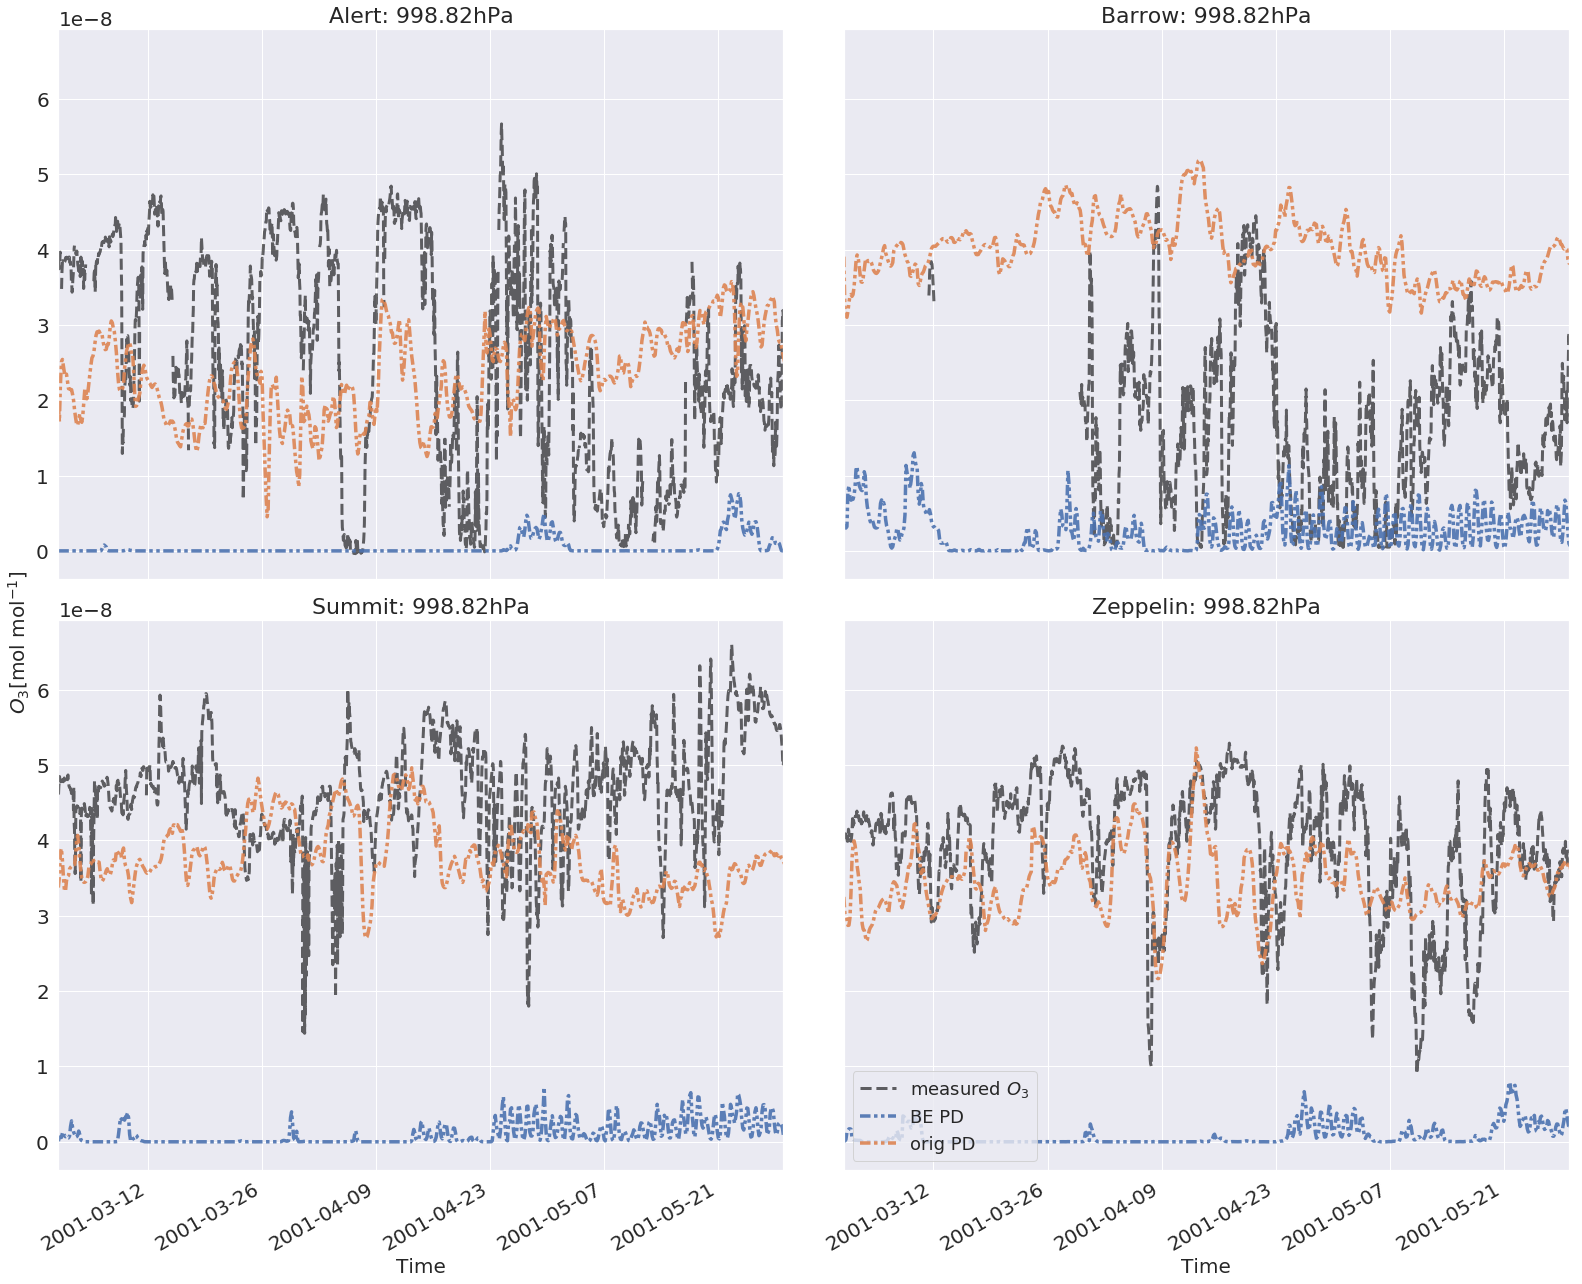
\includegraphics[width = \linewidth]{Chapter6_Results/images/ozone_2001_compObsOrigBE.png}
    \caption{Caption}
    \label{fig:CompObsOrigBE}
\end{figure}



\subsection{Test: Removing Heterogeneous Reactions}

Figure \ref{fig:test_RemoveHetReacts} shows results in terms of $\chem{O_3}$-concentration from attempting to turn off different heterogeneous reactions, namely snow/ice reactions (described in Section \ref{sec:snow_ice_react}), heterogeneous reactions over aerosol surfaces (described in Section \ref{sec:aerosol_react}) as well as heterogeneous reactions involving chlorine and bromine, respectively. The runs were initiated with the same restart file (spin-up) as Branch \ref{def:BE_PD}. For this purpose, four new branches were created (for a full overview of the branches, see Table \ref{tab:branches}). These were:

\begin{mydef}\label{def:BE_PD_noAerosol}
    \texttt{marikoll\_bromine\_explosion\_noHetAerosol}: Branch \ref{def:BE_PD} without heterogeneous aerosol reactions (Reaction \ref{R:8}). 
\end{mydef}

\begin{mydef}\label{def:BE_PD_noIce}
    \texttt{marikoll\_bromine\_explosion\_noSnowIce}: Branch \ref{def:BE_PD} without heterogeneous reactions over ice surfaces (called \texttt{noSnowIce} by mistake) (Reaction \ref{R:7}).
\end{mydef}

\begin{mydef}\label{def:BE_PD_noCl}
    \texttt{marikoll\_bromine\_explosion\_noHetChlorine}: Branch \ref{def:BE_PD} without heterogeneous reactions involving chlorine (Reaction \ref{R:8} and \ref{R:7} with $\chem{X} = \chem{Cl}$).
\end{mydef}

\begin{mydef}\label{def:BE_PD_noBr}
    \texttt{marikoll\_bromine\_explosion\_noHetBromine}: Branch \ref{def:BE_PD} without heterogeneous reactions involving bromine (Reaction \ref{R:8} and \ref{R:7} with $\chem{X} = \chem{Br}$).
\end{mydef}


\begin{table}
\centering
\begin{tabular}{|ll|}
\hline
\textbf{Branch}                                      & \textbf{Reference}          \\ \hline
\texttt{marikoll\_originalCTM3\_NoStrat}             & \ref{def:origCTM3_PD}     \\
\texttt{marikoll\_originalCTM3\_noStrat\_pi}         & \ref{def:origCTM3_PI}     \\
\texttt{marikoll\_bromine\_explosion\_susanne}       & \ref{def:BE_PD}           \\
\texttt{marikoll\_bromine\_explosion\_PI}            & \ref{def:BE_PI}           \\
\texttt{marikoll\_bromine\_explosion\_noHetAerosol}  & \ref{def:BE_PD_noAerosol} \\
\texttt{marikoll\_bromine\_explosion\_noSnowIce}     & \ref{def:BE_PD_noIce}     \\
\texttt{marikoll\_bromine\_explosion\_noHetChlorine} & \ref{def:BE_PD_noCl}      \\
\texttt{marikoll\_bromine\_explosion\_noHetBromine}  & \ref{def:BE_PD_noBr}      \\ \hline
\end{tabular}
\caption{Overwiew of brances used in the developing process. References refer to chapter and branch number}
\label{tab:branches}
\end{table}


\begin{figure}
    \centering
    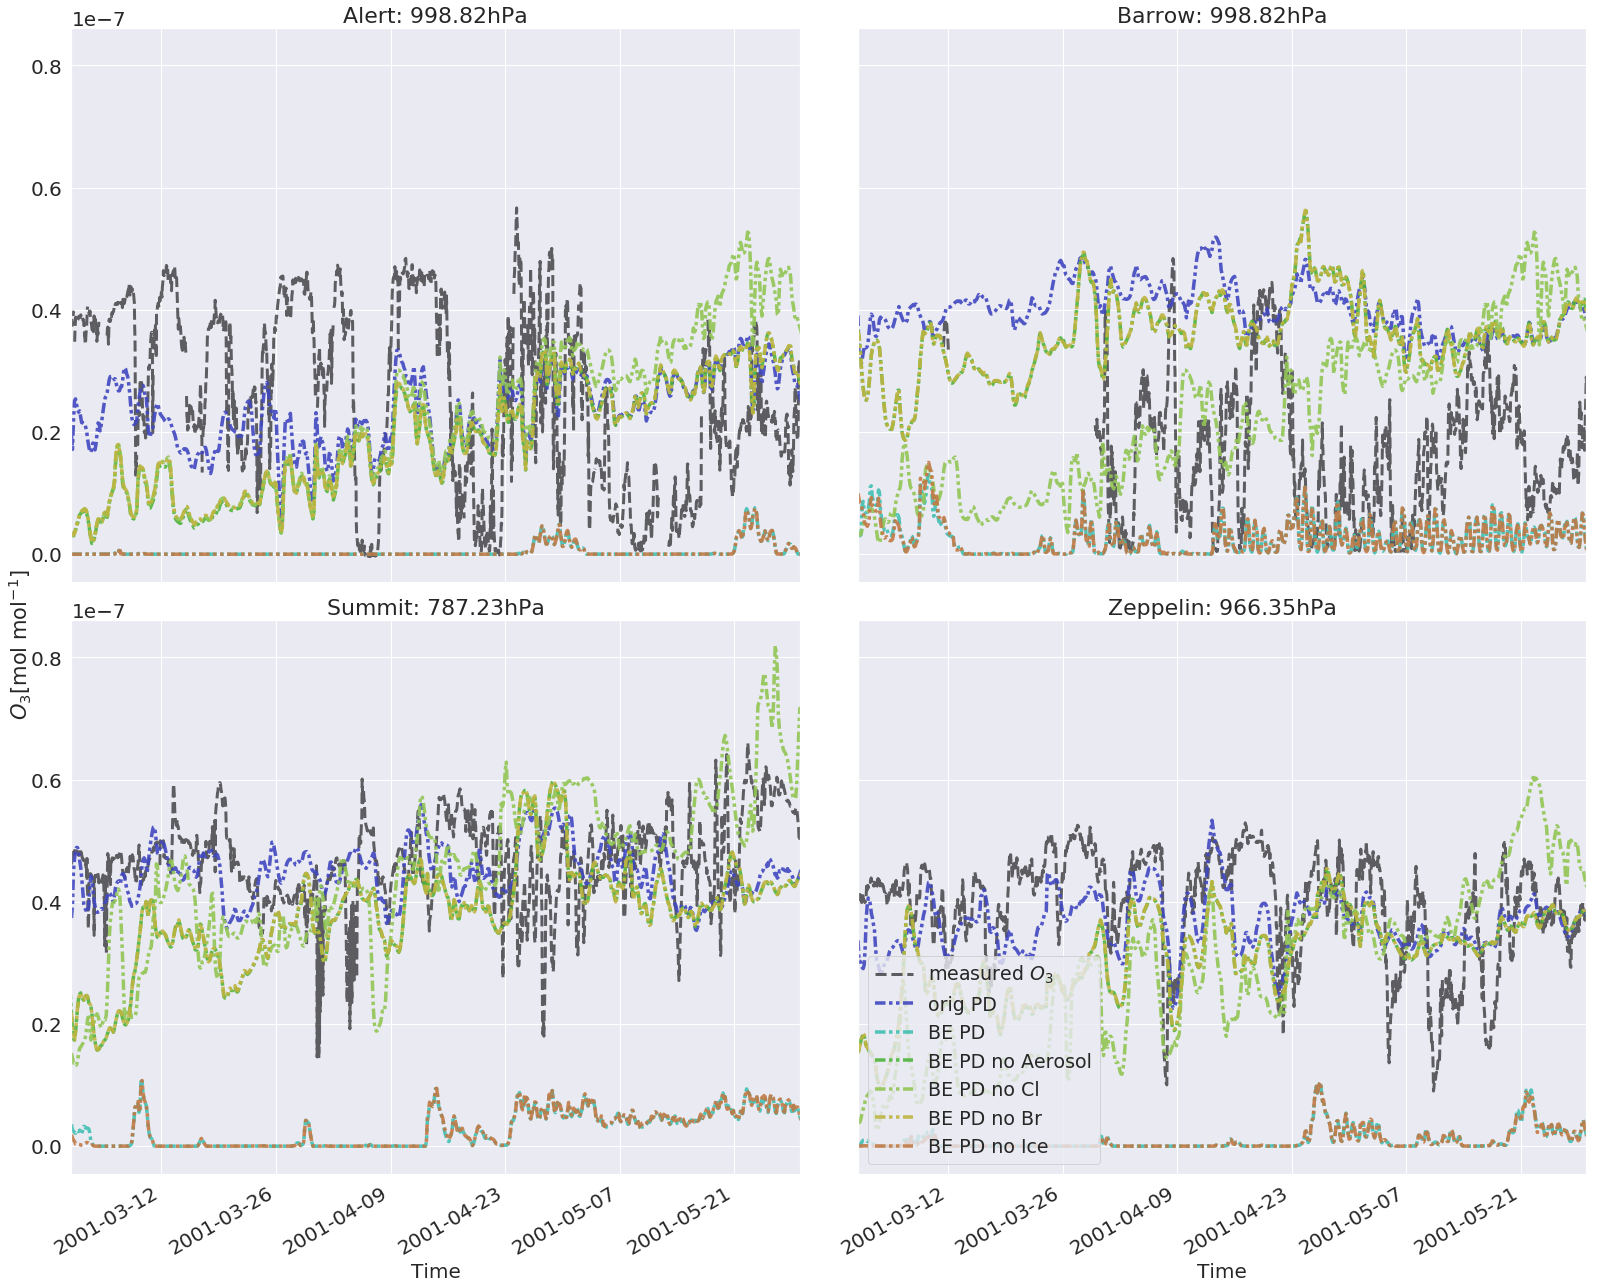
\includegraphics[width = \linewidth]{Chapter6_Results/images/ozone_removingHetReacts.png}
    \caption{Ozone measurements (black line) and model results from the original CTM3 (blue line), Branch \ref{def:BE_PD} (turquoise line), Branch \ref{def:BE_PD_noAerosol} (green line), \ref{def:BE_PD_noIce} (orange line), Branch \ref{def:BE_PD_noCl} (light green line) and Branch \ref{def:BE_PD_noBr} (yellow line) at the four different stations, Alert (top left), Barrow (top right), Summit (lower left) and Zeppelin (lower right) with available measurements in 2001. Model results were taken from the approximate altitude of the station in hPa. PD = present day, BE = bromine explosion}
    \label{fig:test_RemoveHetReacts}
\end{figure}


\medskip

Figure \ref{fig:vertHBr_noCl} shows the vertical column above the Alert, Barrow, Summit and Zeppelin of the mixing ratio of \chem{HBr}. The mixing ratio is on the order $10^{-15}$ (0.001 ppt). The vertical distribution appears to be constrained with higher concentration in the lower layers at Alert, whilst increasing with altitude at Zeppelin. Seen in relation with Figure \ref{fig:polarHBr_noCl}, the concentration in the lowest layer across the Arctic is on the order of $10^{-10} - 10^{-11} g m^{-3}$

\medskip

In Figure \ref{fig:polarBrO_noCl}, the vertical column density for the lowermost $\sim$ 250 m is plotted. The column density is on the order $10^{6}$ molecules cm$^{-2}$

%In the vertical, the corresponding $\chem{Br_y}$ concentrations to Figure \ref{fig:test_RemoveHetReacts} are shown in Figures \ref{fig:vert_noAer_bry_2001}-\ref{fig:vert_noBr_bry_2001} for the four new branches, Branch \ref{def:BE_PD_noAerosol}-\ref{def:BE_PD_noBr}, respectively (The $\chem{Br_y}$-family is explained in Section \ref{sec:halogen_families_BryClxCly}). 

\begin{figure}[ht]
    \centering
    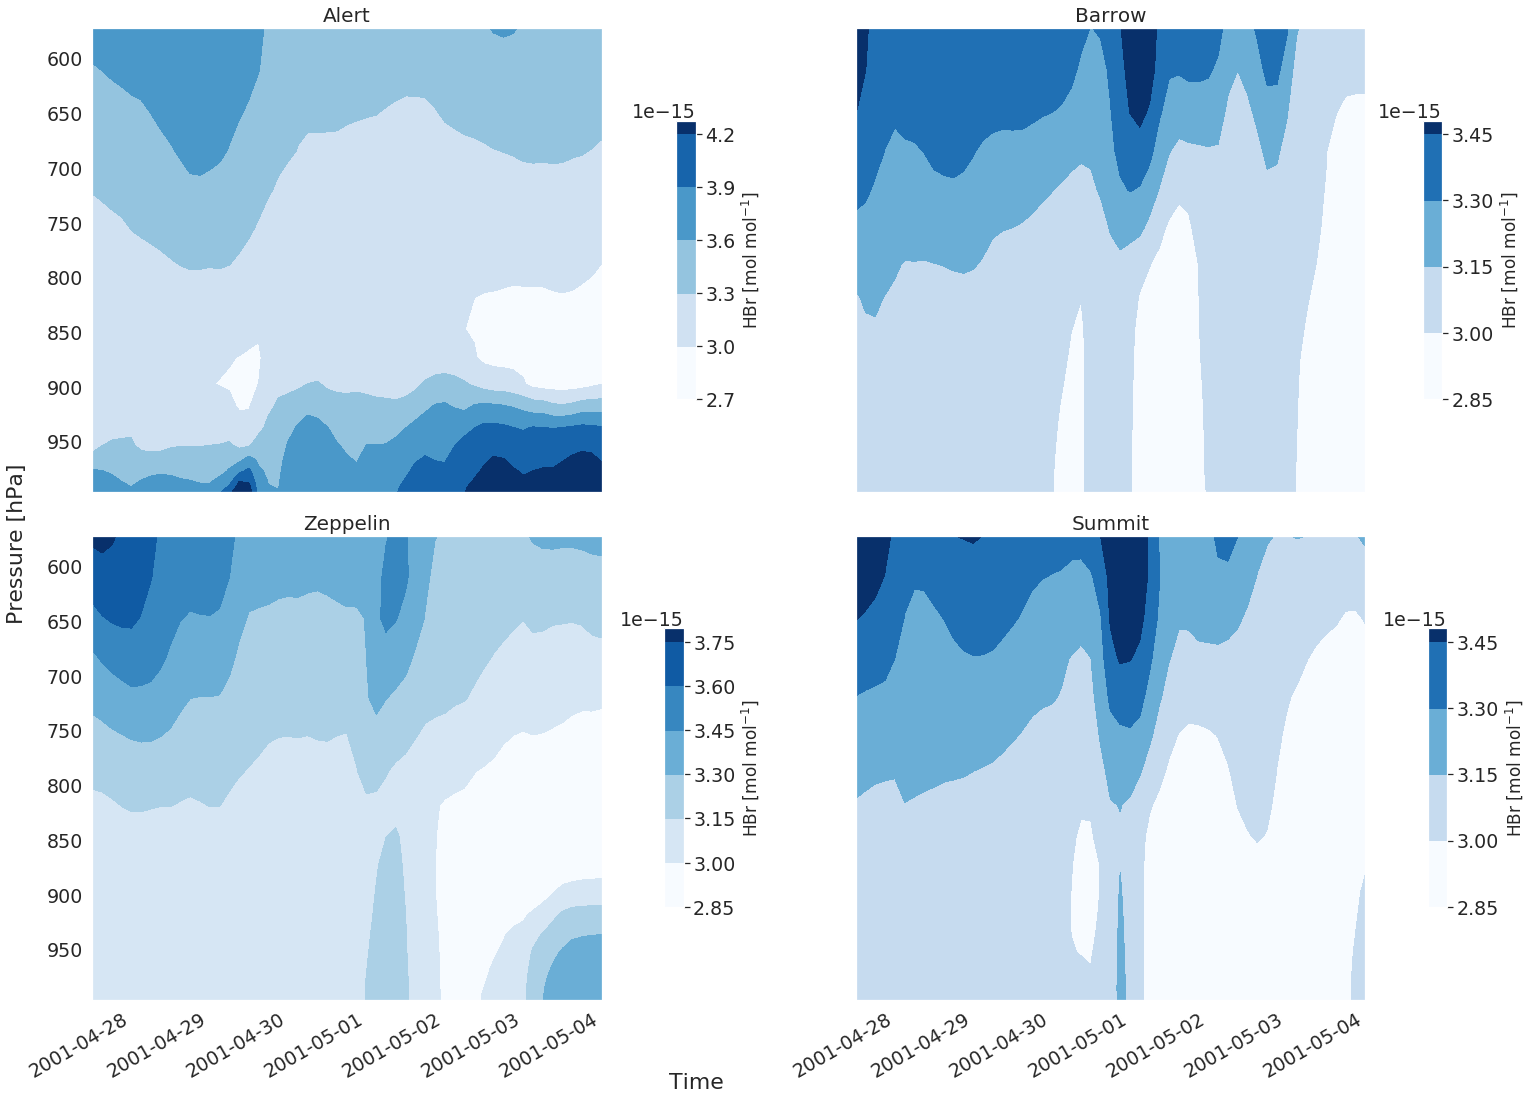
\includegraphics[width = \linewidth]{Chapter6_Results/images/vertHBr_noCl.png}
    \caption{Mixing ratio ($mol mol^{-1}$) of \chem{HBr} in the model layers up to $\sim 600 hPa$ at the four different stations Alert (top left), Barrow (top right), Zeppelin (lower left) and Summit (lower right) in April-May, 2001. The result is from Branch \ref{def:BE_PD_noCl}}
    \label{fig:vertHBr_noCl}
\end{figure}

\begin{figure}[h]
    \centering
    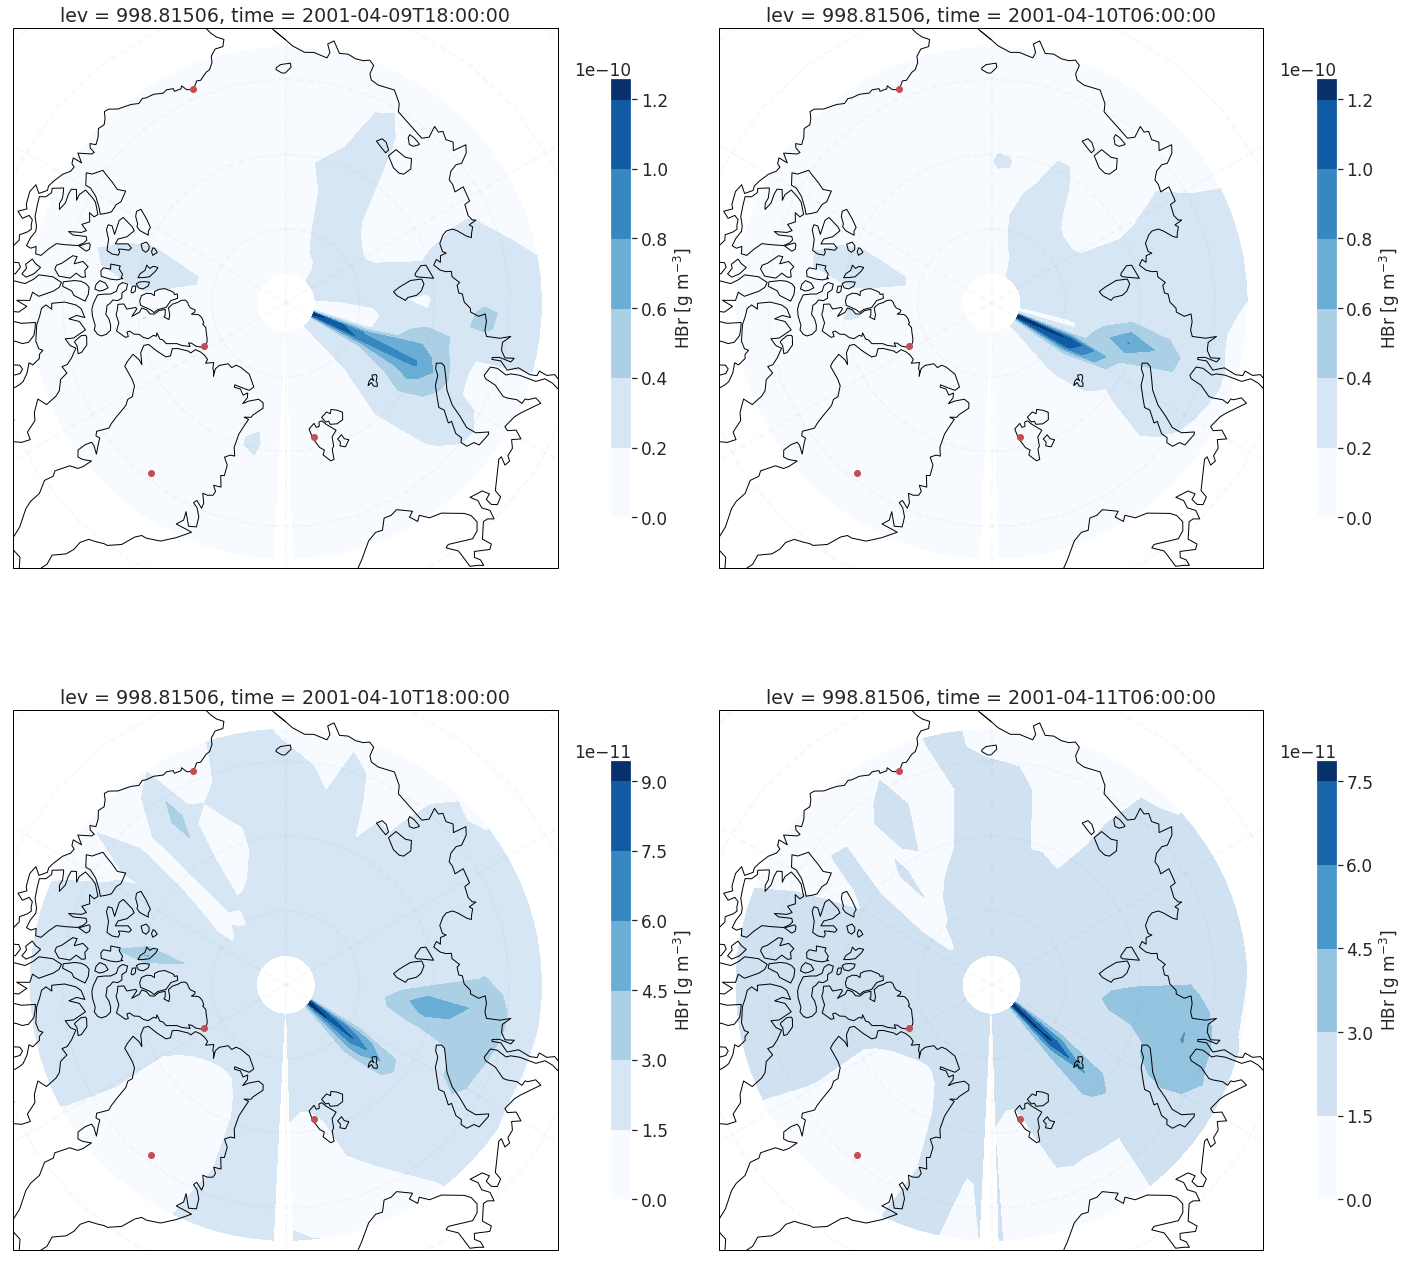
\includegraphics[width = \linewidth]{Chapter6_Results/images/polarHBr_noCl.png}
    \caption{Concentration ($g m^{-3}$) of \chem{HBr} in the first model layer the Arctic at 18:00 and 06:00 (UTC) of the 9th, 10th and 11th of April, 2001. The result is from Branch \ref{def:BE_PD_noCl} The red dots are the positions of the stations with observations in 2001 (see the map in Figure \ref{fig:stns} for reference)}
    \label{fig:polarHBr_noCl}
\end{figure}

\begin{figure}[ht]
    \centering
    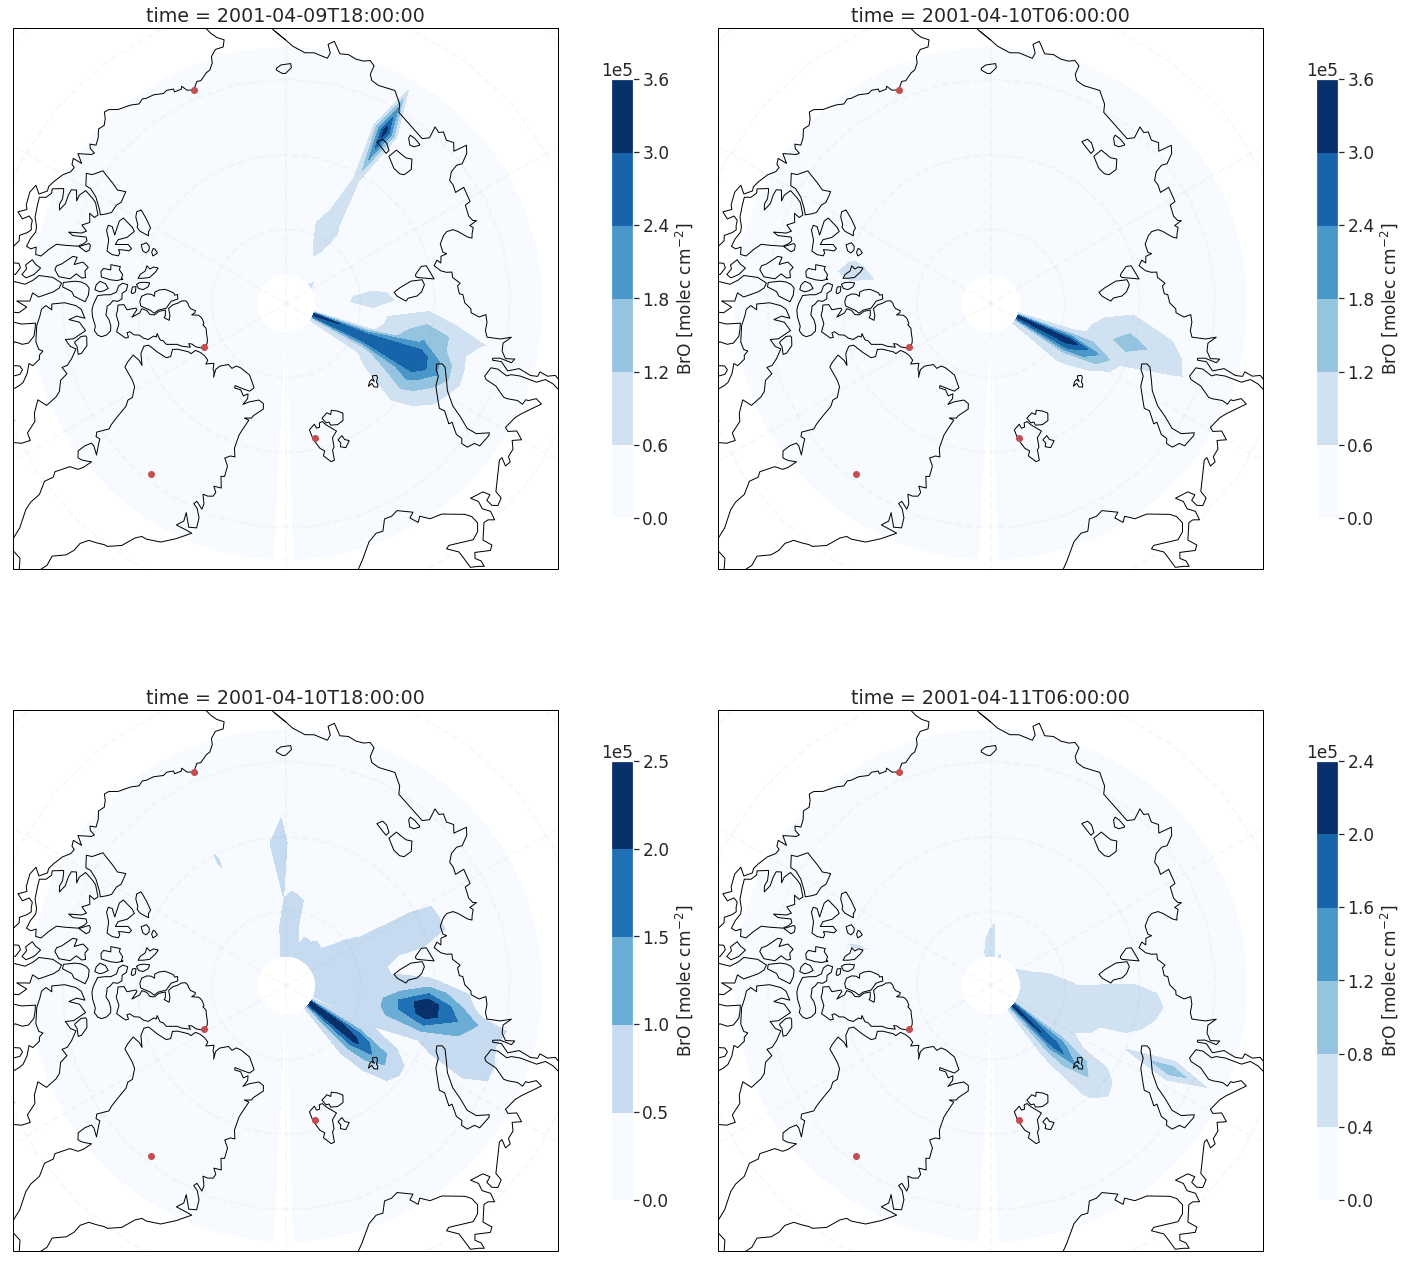
\includegraphics[width = \linewidth]{Chapter6_Results/images/polarBrO_noCl.png}
    \caption{Vertical column density ($molecules cm^{-2}$) of \chem{BrO} in the lowermost $\sim 250 m$ at in the morning and evening (UTC) on the 9th and 10th of April, 2001. The result is from Branch \ref{def:BE_PD_noCl}. The red dots are the positions of the stations with observations in 2001 (see the map in Figure \ref{fig:stns}}
    \label{fig:polarBrO_noCl}
\end{figure}

%\begin{figure}
    \centering
    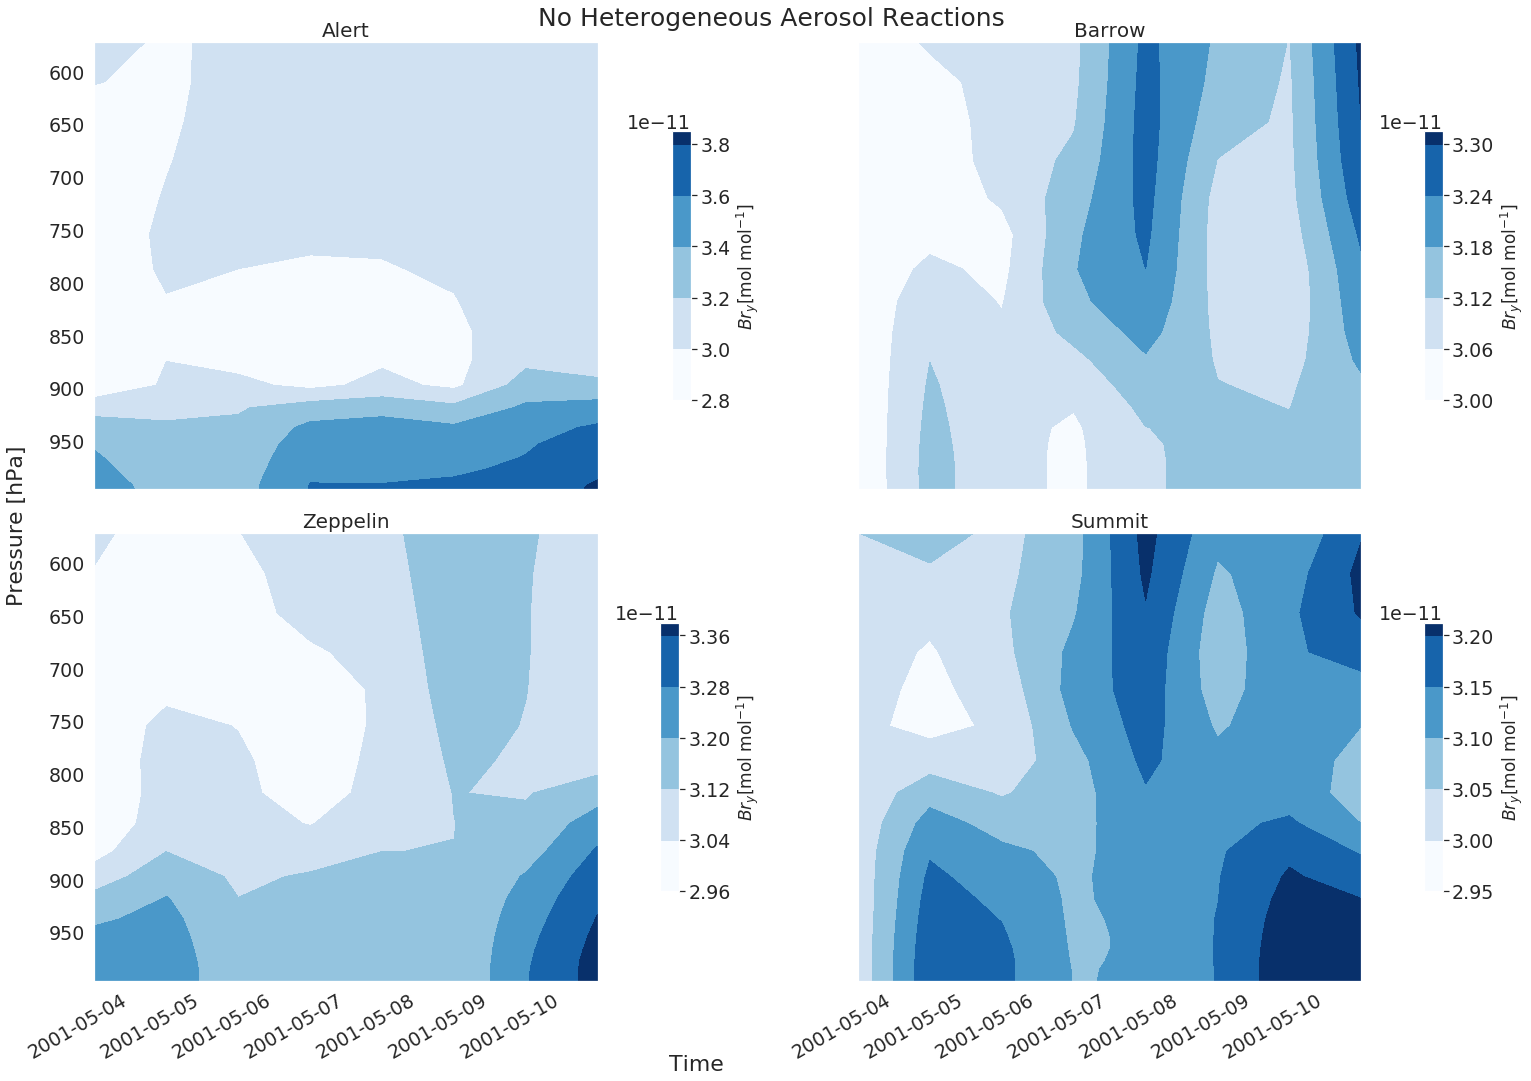
\includegraphics[width = \linewidth]{Chapter6_Results/images/noAerosol_2001_bry.png}
    \caption{Modelled $\chem{Br_y}$ without the heterogeneous aerosol reactions. The y-axis shows altitude up to 600 hPa at each station with ozone measurements at 12:00 (UTC) (Alert, Barrow, Zeppelin and Summit) in 2001.}
    \label{fig:vert_noAer_bry_2001}
\end{figure}

%\begin{figure}
    \centering
    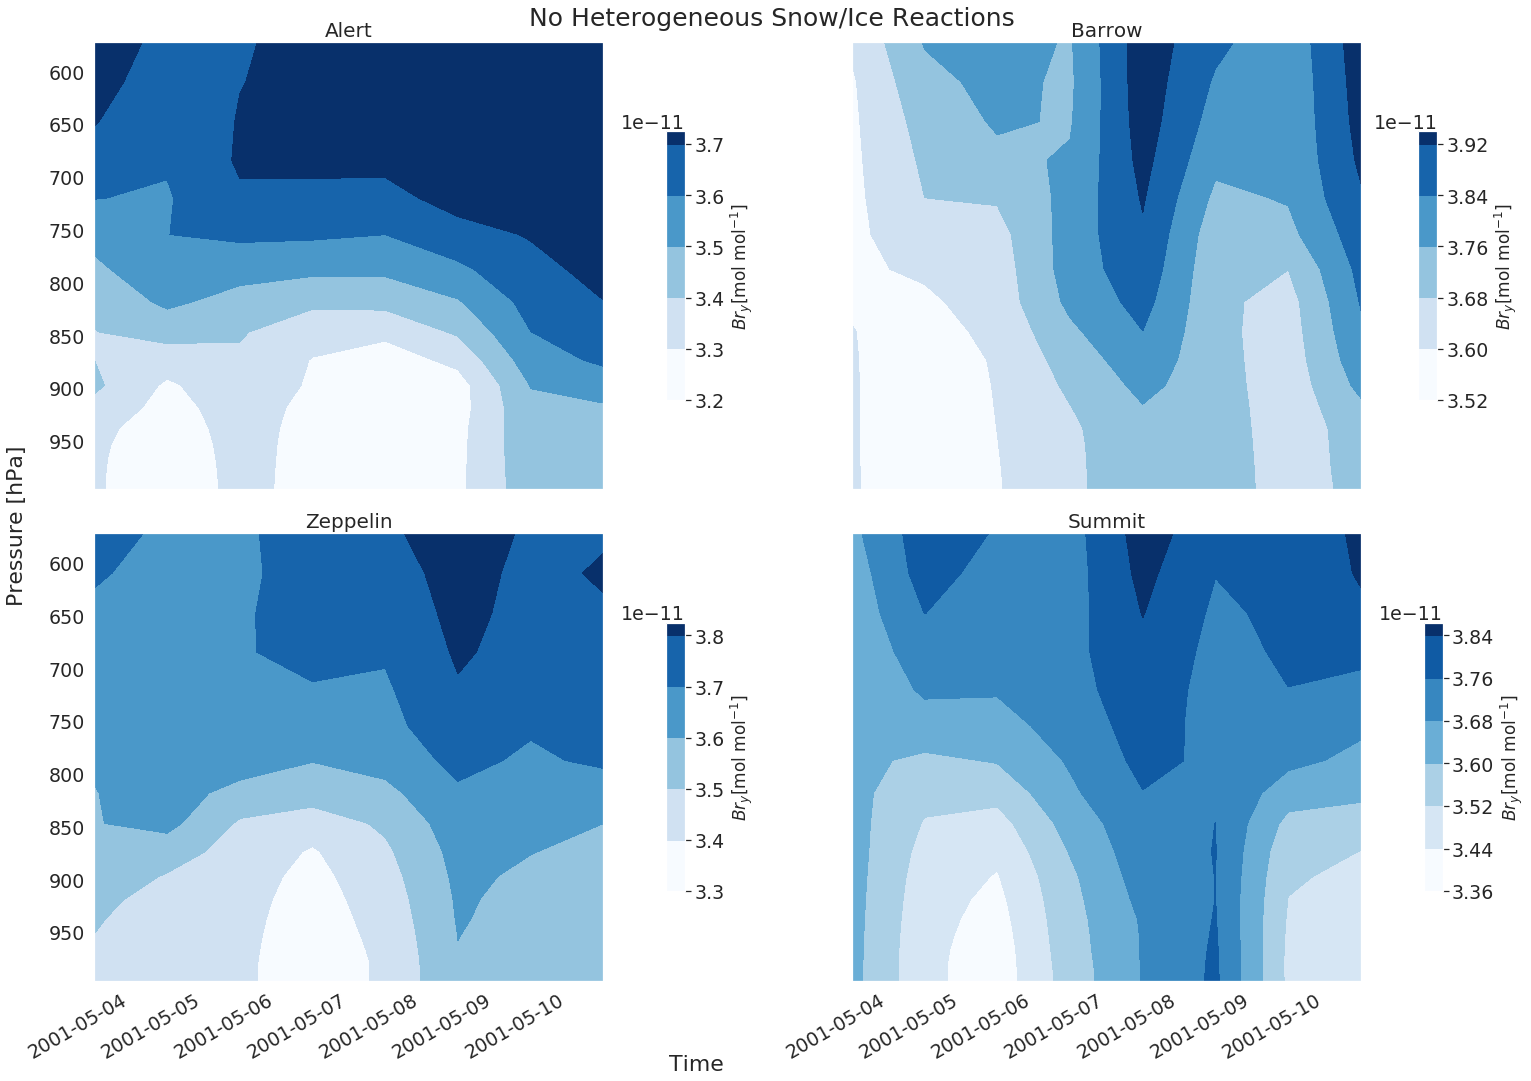
\includegraphics[width = \linewidth]{Chapter6_Results/images/noSnowIce_2001_bry.png}
    \caption{Modelled $\chem{Br_y}$ without theheterogeneous reactions over ice surfaces. The y-axis shows altitude up to 600 hPa at each station with ozone measurements (Alert, Barrow, Zeppelin and Summit) in 2001.}
    \label{fig:vert_noSnowIce_bry_2001}
\end{figure}

%\begin{figure}
    \centering
    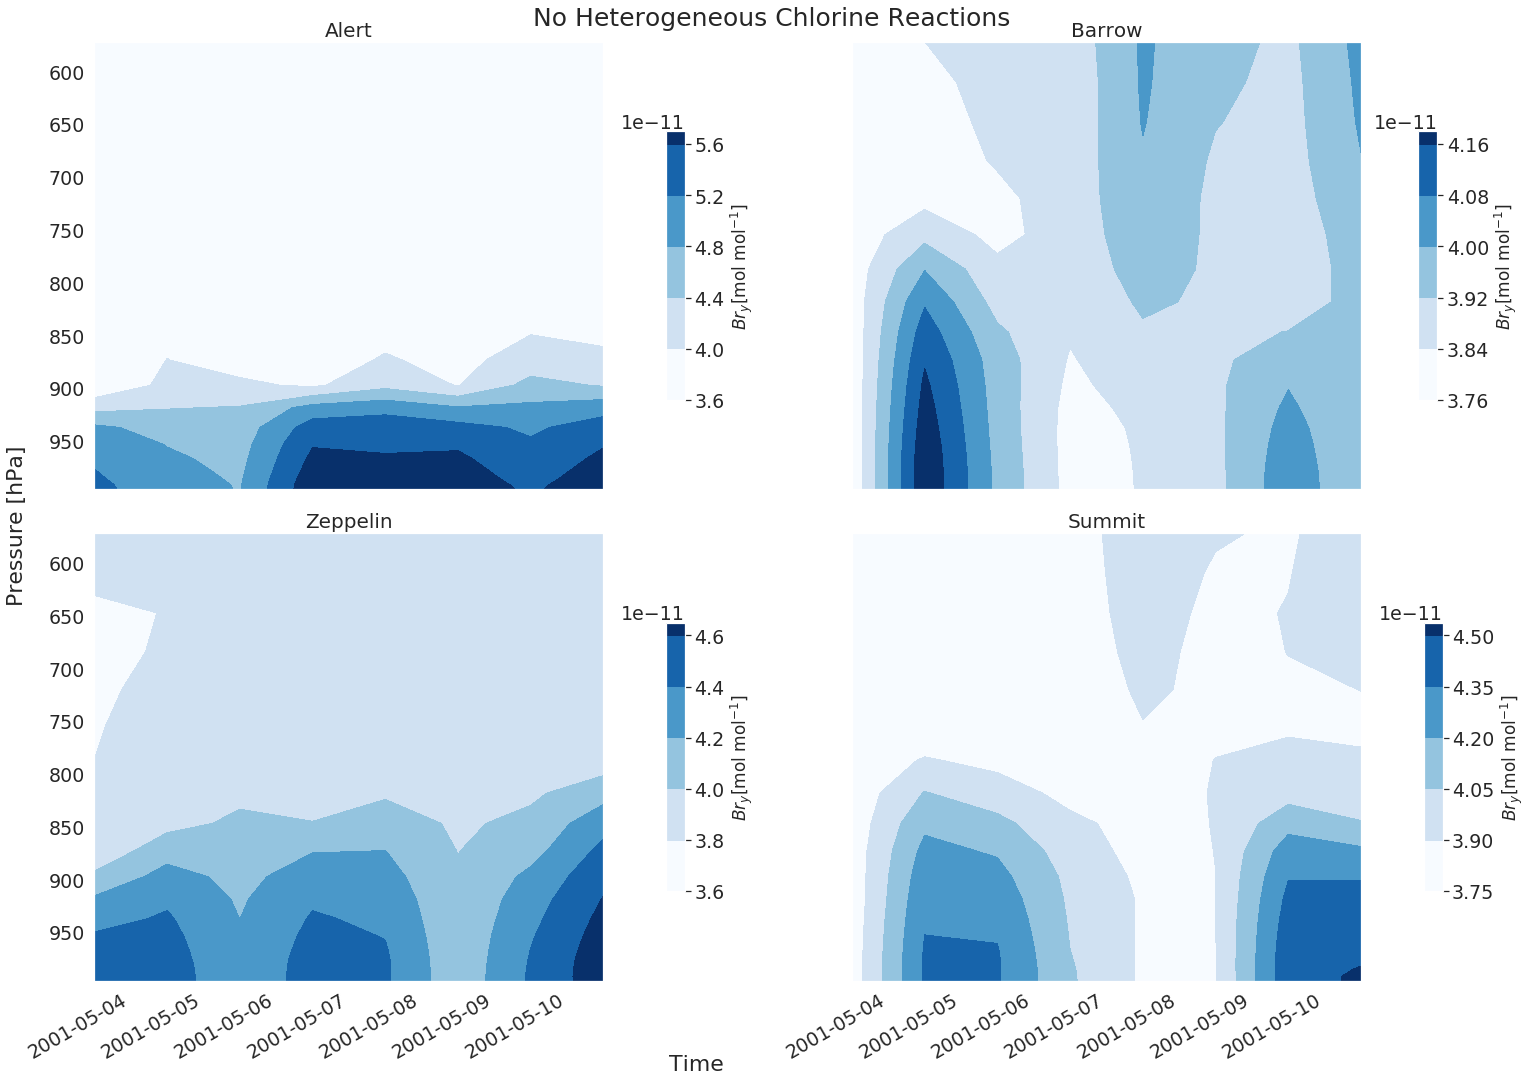
\includegraphics[width = \linewidth]{Chapter6_Results/images/noCl_2001_bry.png}
    \caption{Modelled $\chem{Br_y}$ without the heterogeneous reactions involving chlorine. The y-axis shows altitude up to 600 hPa at each station with ozone measurements (Alert, Barrow, Zeppelin and Summit) in 2001.}
    \label{fig:vert_noCl_bry_2001}
\end{figure}

%\begin{figure}
    \centering
    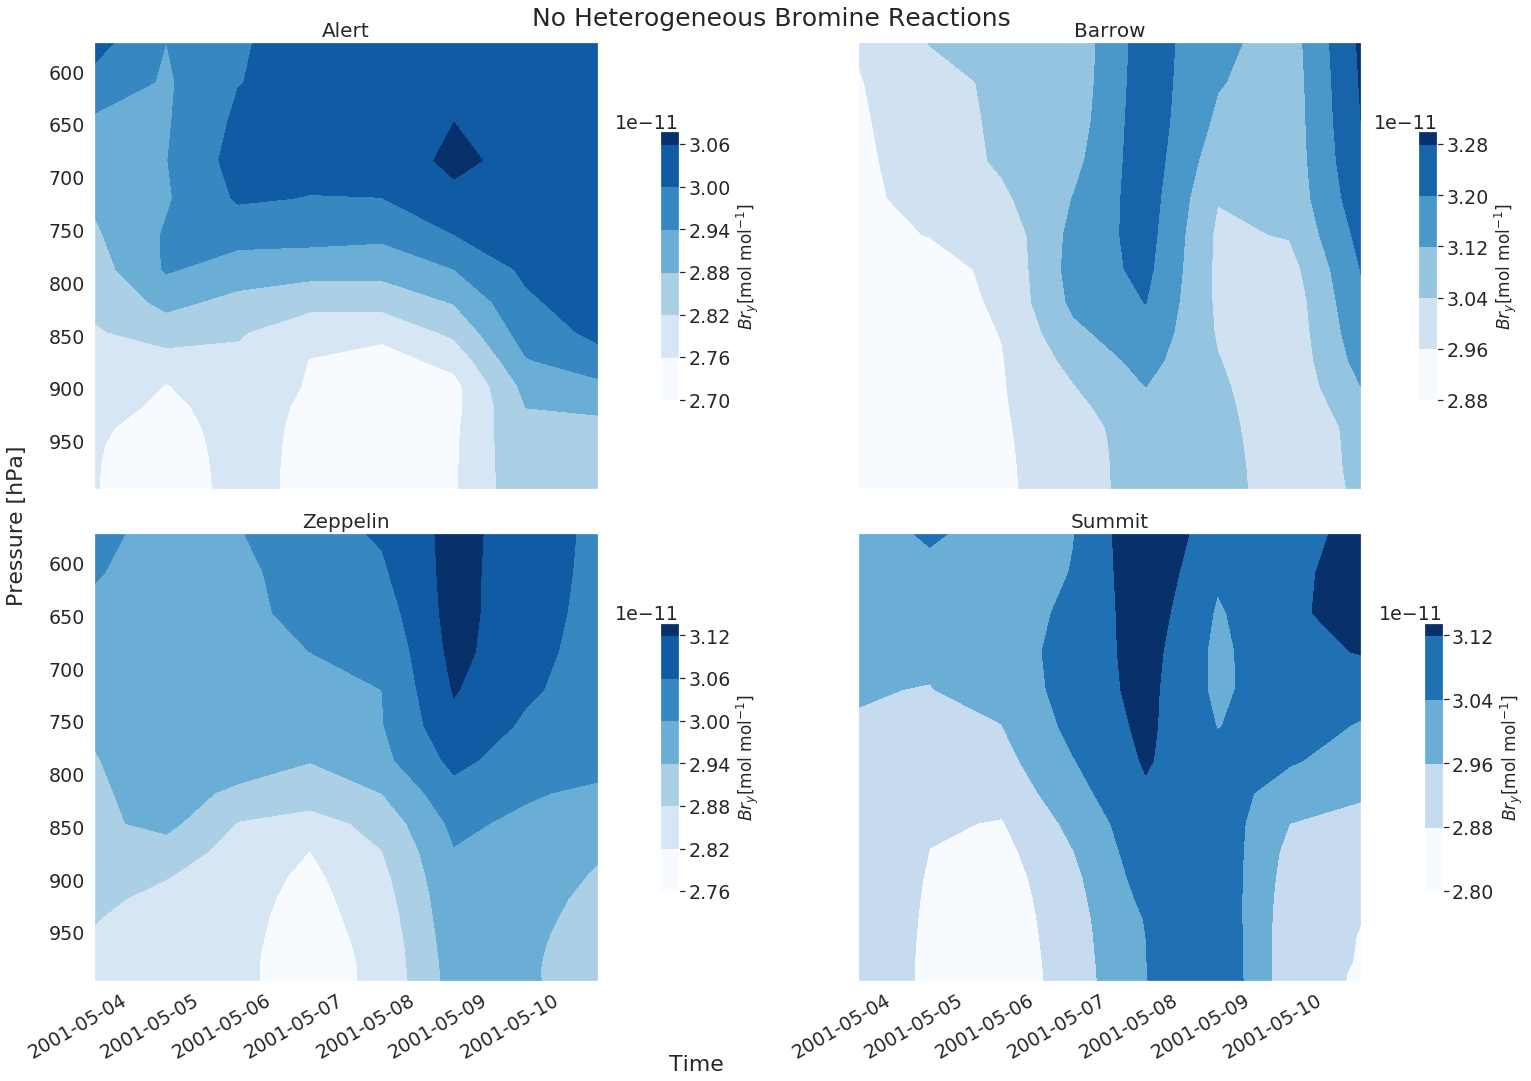
\includegraphics[width = \linewidth]{Chapter6_Results/images/noBr_2001_bry.png}
    \caption{Modelled $\chem{Br_y}$ without the heterogeneous reactions involving bromine. The y-axis shows altitude up to 600 hPa at each station with ozone measurements at 12:00 (UTC) (Alert, Barrow, Zeppelin and Summit) in 2001.}
    \label{fig:vert_noBr_bry_2001}
\end{figure}




%\textbf{NOTE:} after these tests, a mistake in the scaling of $\chem{Cl_x}$ was discovered. \chem{BrCl} had mistakenly been scaled with this family, which led to disappearance of all \chem{Cl}-species. The subsequent tests were fixed for this.

%\subsection{Integrating $\chem{Cl_y}$ in Branch \ref{def:BE_PD}}

%Figure \ref{fig:test_ClyInt} contains the result in terms of $\chem{O_3}$ concentration where an integration of the $\chem{Cl_y}$-family was added to the initial BE-branch (Branch \ref{def:BE_PD}) This integration was not handled prior to the previous model runs (the chemical families are listed in Section \ref{sec:halogen_families_BryClxCly}). 

%\medskip

%As the inclusion of $\chem{ClONO2}$ (Reaction \ref{R:clono2}) function purely as a sink to the $\chem{ClO}$, this reaction was also removed altogether to see if this would help the low chlorine levels. 

%\begin{figure}
    \centering
    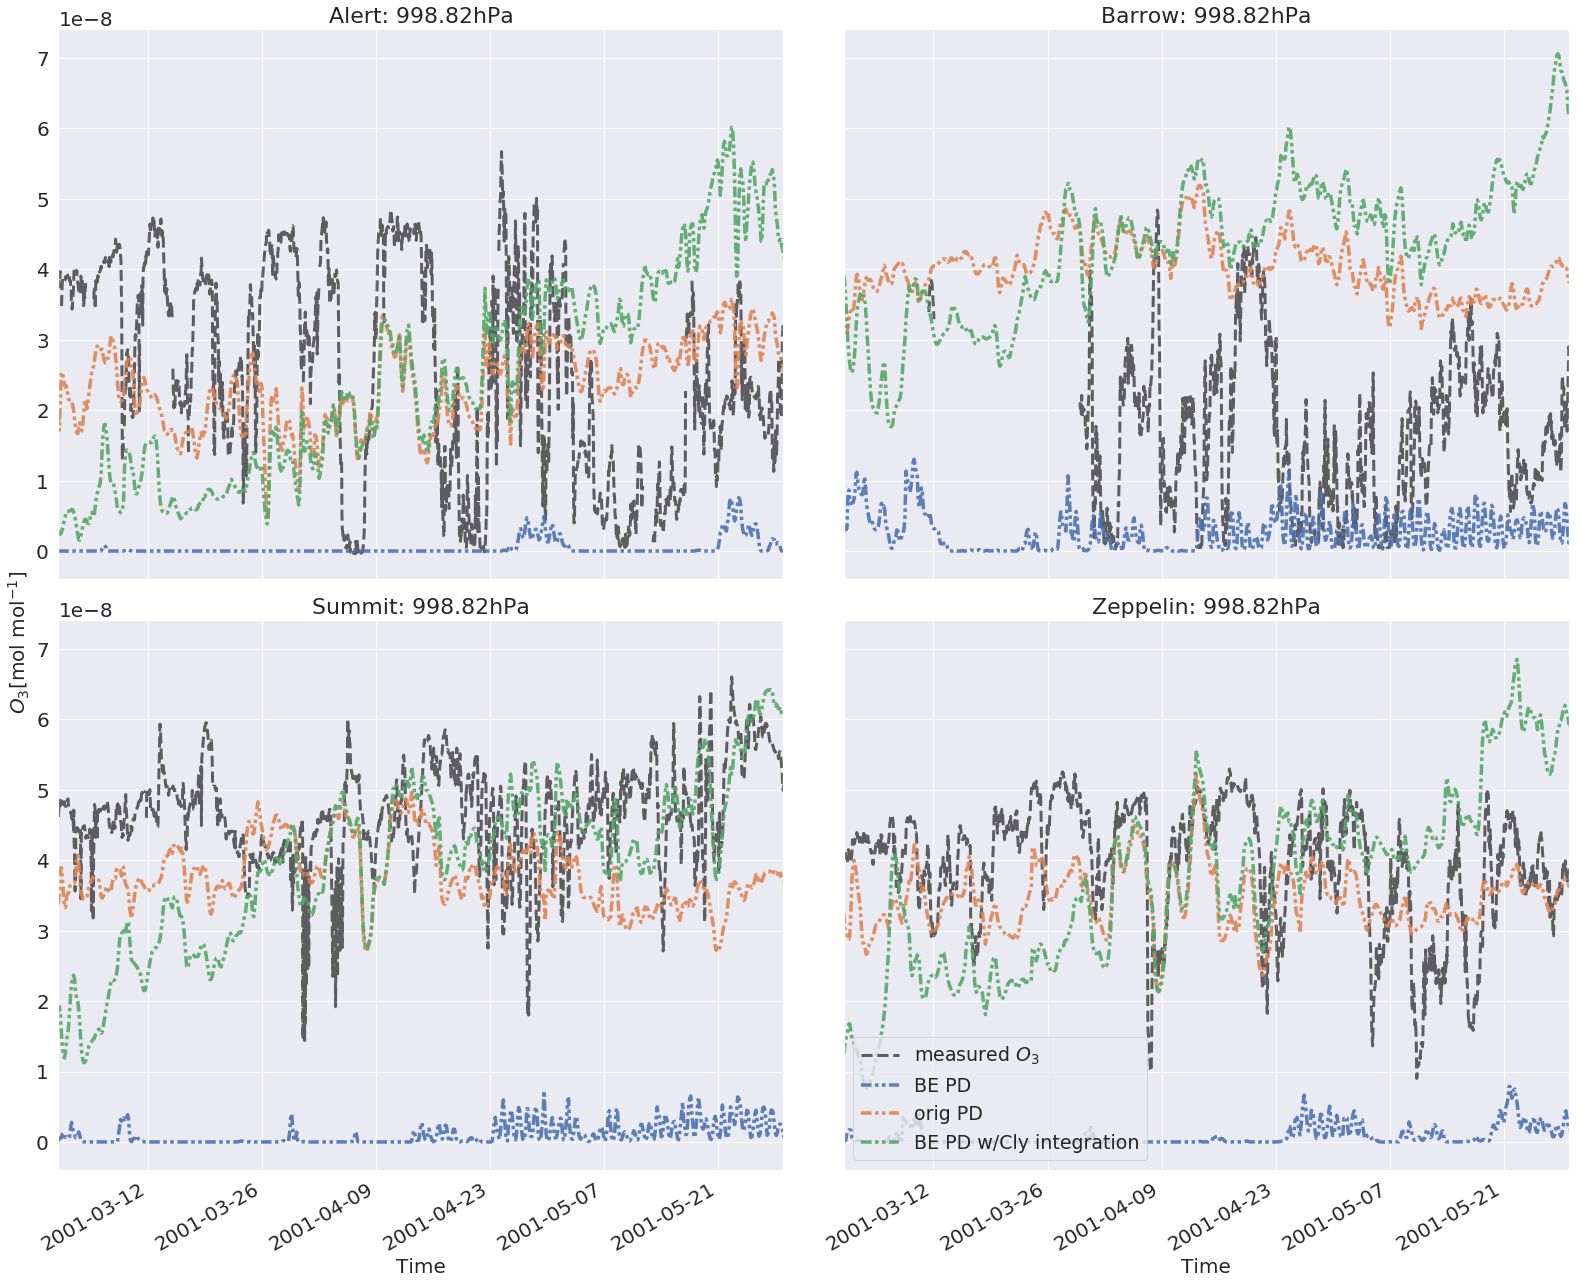
\includegraphics[width = \linewidth]{Chapter6_Results/images/ozone_2001_newClyIntegration.png}
    \caption{Ozone measurements (black line) and model results from the original CTM3 (orange line), Branch \ref{def:BE_PD} (blue line) and the attempt to integrate the $\chem{Cl_y}$ family (green line) at the four different stations, Alert (top left), Barrow (top right), Summit (lower left) and Zeppelin (lower right) with available measurements in 2001. Model results are taken from the first model level at $998.82 hPa$. PD = present day, BE = bromine explosion}
    \label{fig:test_ClyInt}
\end{figure}

\clearpage

\subsection{Development of Branch \ref{def:BE_PD_noCl} Without Heterogeneous Chlorine Reactions}\label{sec:res_noHetCl}

\subsubsection{Initializing Branch \ref{def:BE_PD_noCl} With a Higher \chem{HBr} Concentration}\label{sec:res_step2}

In order to boost the concentration of \chem{HBr}, the concentration was hard-coded to 30 ppt ($= 8.059\cdot10^8 \text{molecules}cm^{-3}$ at $273.15 K$) and 10 ppt ($= 2.69\cdot10^8 \text{molecules}cm^{-3}$ at $273.15 K$), respectively, in the first sub-timestep of \texttt{pchemc\_ij.f90}. Further, a run initialized with a restart file from the 10 ppt run was performed in which the hard-coded concentration of \chem{HBr} was removed.

\medskip

Figure \ref{fig:ozone_noCl_step2} contains results from different attempts to boost the \chem{HBr}-concentration, to see the effect on ozone depletion. The first test, in which the concentration of \chem{HBr} was constantly boosted by hard-coding to maintain 30 ppt (green line), results in mixing ratios of $\chem{O_3}$ comparable to the original CTM3-branch (blue line). In the second test, the \chem{HBr}-concentration was hard-coded to 10 ppt (light green line), which results in concentrations more comparable to the measurements. Lastly, the test in which the run was initiated with a restart file from the previous hard-coded test (\chem{HBr} concentration of 10 ppt) (yellow line) also maintains concentrations comparable in magnitude with the observations. All these tests were ran for a short amount of time (2 weeks to a month, model time)

\begin{figure}[ht]
    \centering
    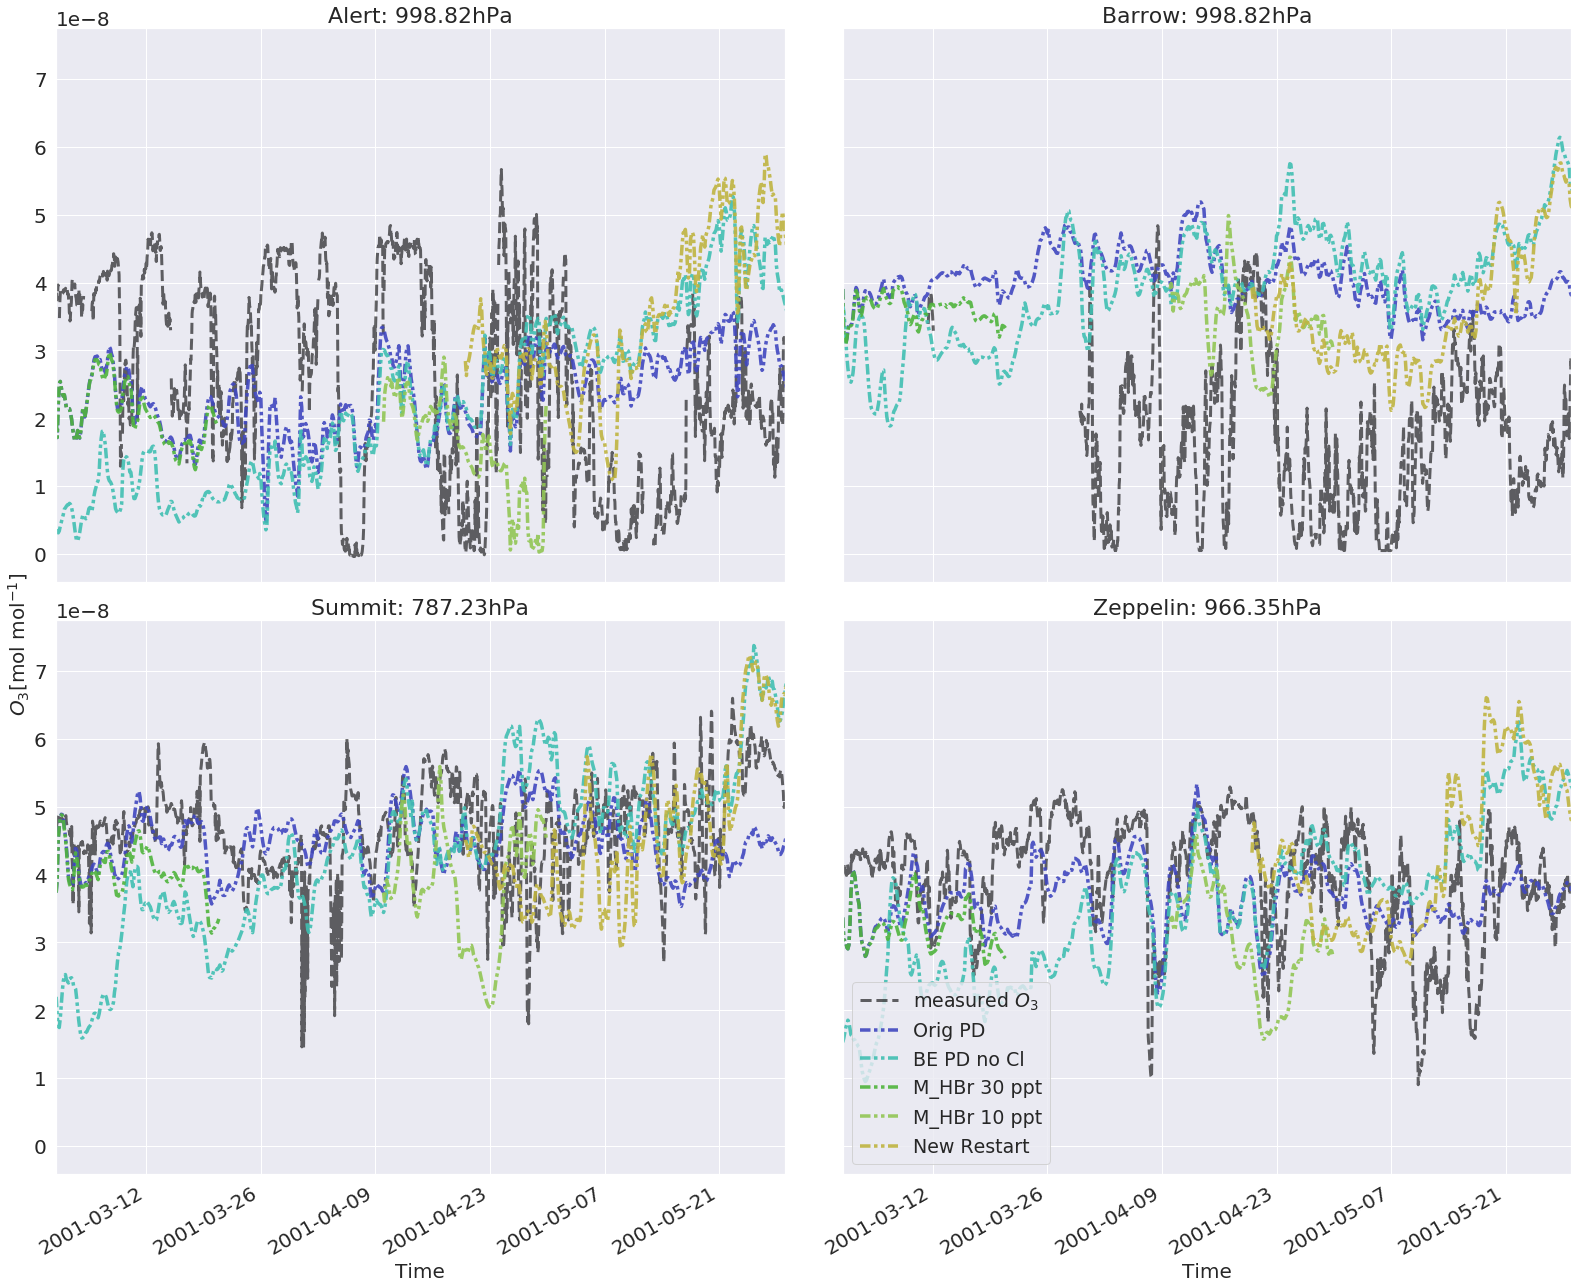
\includegraphics[width=\linewidth]{Chapter6_Results/images/ozone_noCl_step2.png}
    \caption{Ozone measurements (black line) and model results from the original CTM3 (blue line), Branch \ref{def:BE_PD_noCl} (turquoise line) (these three are the same as in Figure \ref{fig:test_RemoveHetReacts}), Branch \ref{def:BE_PD_noCl} with hard coded \chem{HBr}-concentration of 30 ppt (green line), Branch \ref{def:BE_PD_noCl} with hard coded \chem{HBr}-concentration of 10 ppt(light green line) and Branch \ref{def:BE_PD_noCl} initialized with a restart file from the hard coded \chem{HBr}-concentration of 10 ppt- run (yellow line) at the four different stations, Alert (top left), Barrow (top right), Summit (lower left) and Zeppelin (lower right) with available measurements in 2001. Model results are taken from the first model level at $998.82 hPa$. PD = present day, BE = bromine explosion}
    \label{fig:ozone_noCl_step2}
\end{figure}

\medskip

Figure \ref{fig:vertHBr_newRestart} contains the resulting \chem{HBr}-column above Alert, Barrow, Summit and Zeppelin up to approximately $600$ hPa. The mixing ratio is on the order of $25 - 250$ ppt maximum. The higher concentrations appear to be constrained to the lower layers of the troposphere to various extents. In the lowest layer, Figure \ref{fig:polarHBr_newRestart} shows that the concentrations are on the order of $7.5\times10^{-7} - 1.5\times10^{-6}$gm$^{-3}$. Seen in relation with Figure \ref{fig:polarHOBr_newRestart}, \ref{fig:polarHBr_newRestart} is very anti-correlated. 


\begin{figure}[h]
    \centering
    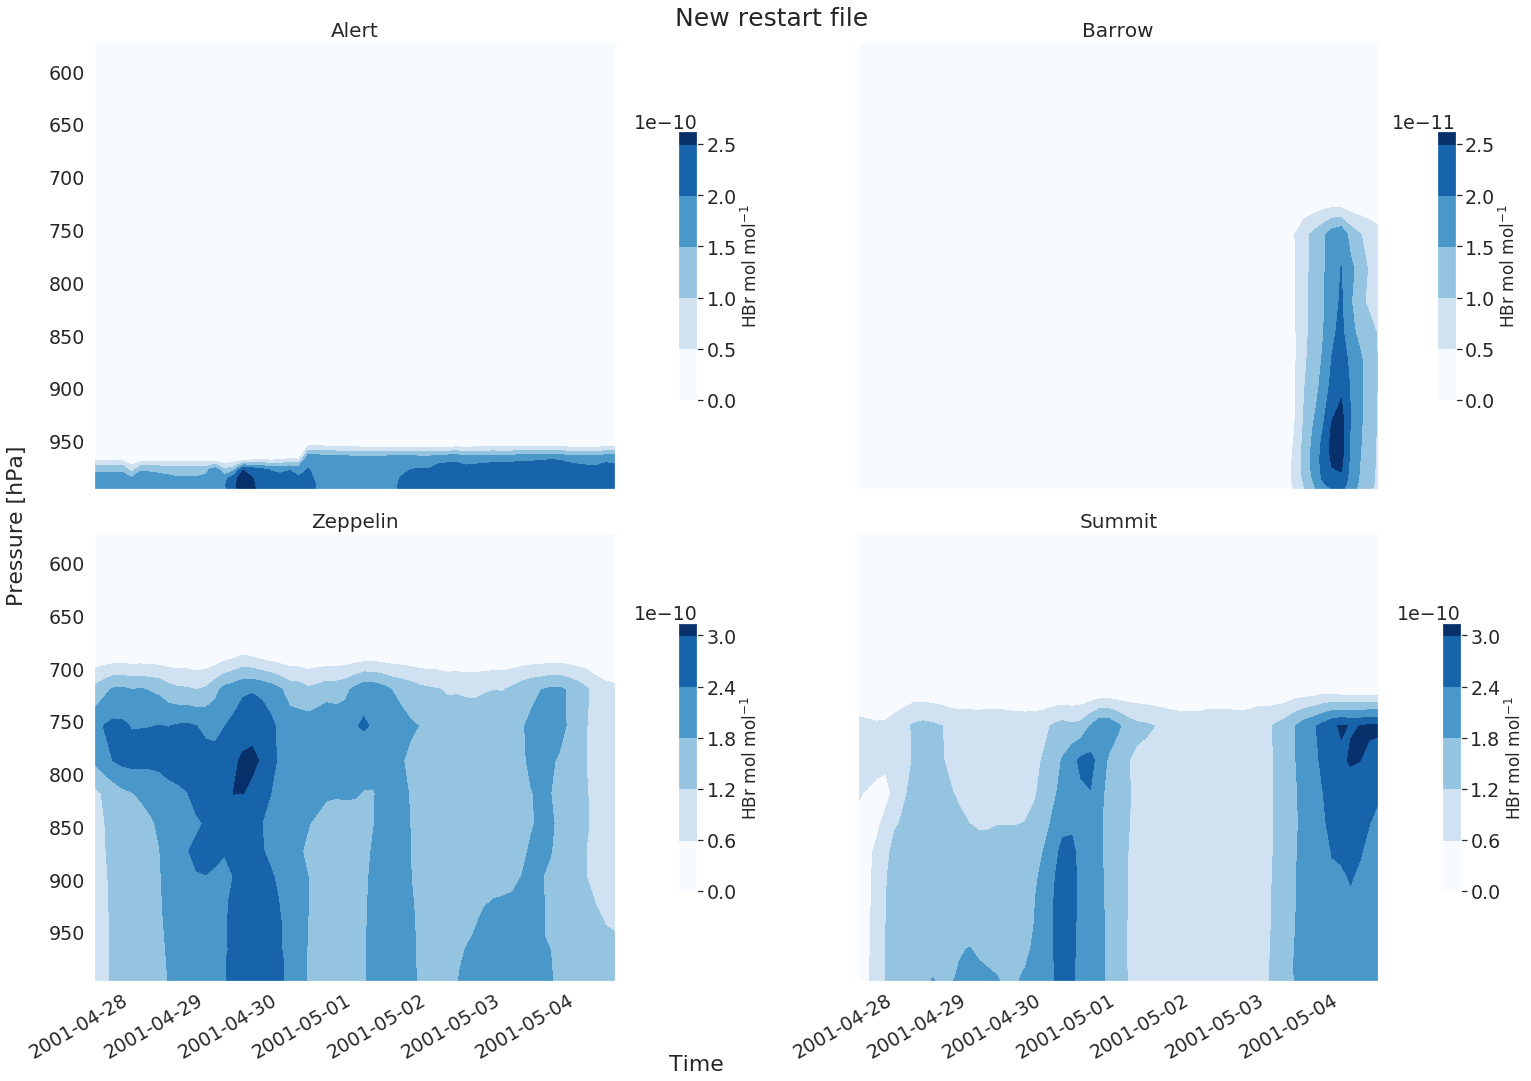
\includegraphics[width=\linewidth]{Chapter6_Results/images/vertHBr_newRestart.png}
    \caption{Mixing ratio ($mol mol^{-1}$) of \chem{HBr} in the model layers up to $\sim 600 hPa$ at the four different stations Alert (top left), Barrow (top right), Zeppelin (lower left) and Summit (lower right) in April, 2001. The result is from Branch \ref{def:BE_PD_noCl} initialized with a new restart file with a \chem{HBr} concentration of 10 ppt}
    \label{fig:vertHBr_newRestart}
\end{figure}

\begin{figure}[h]
    \centering
    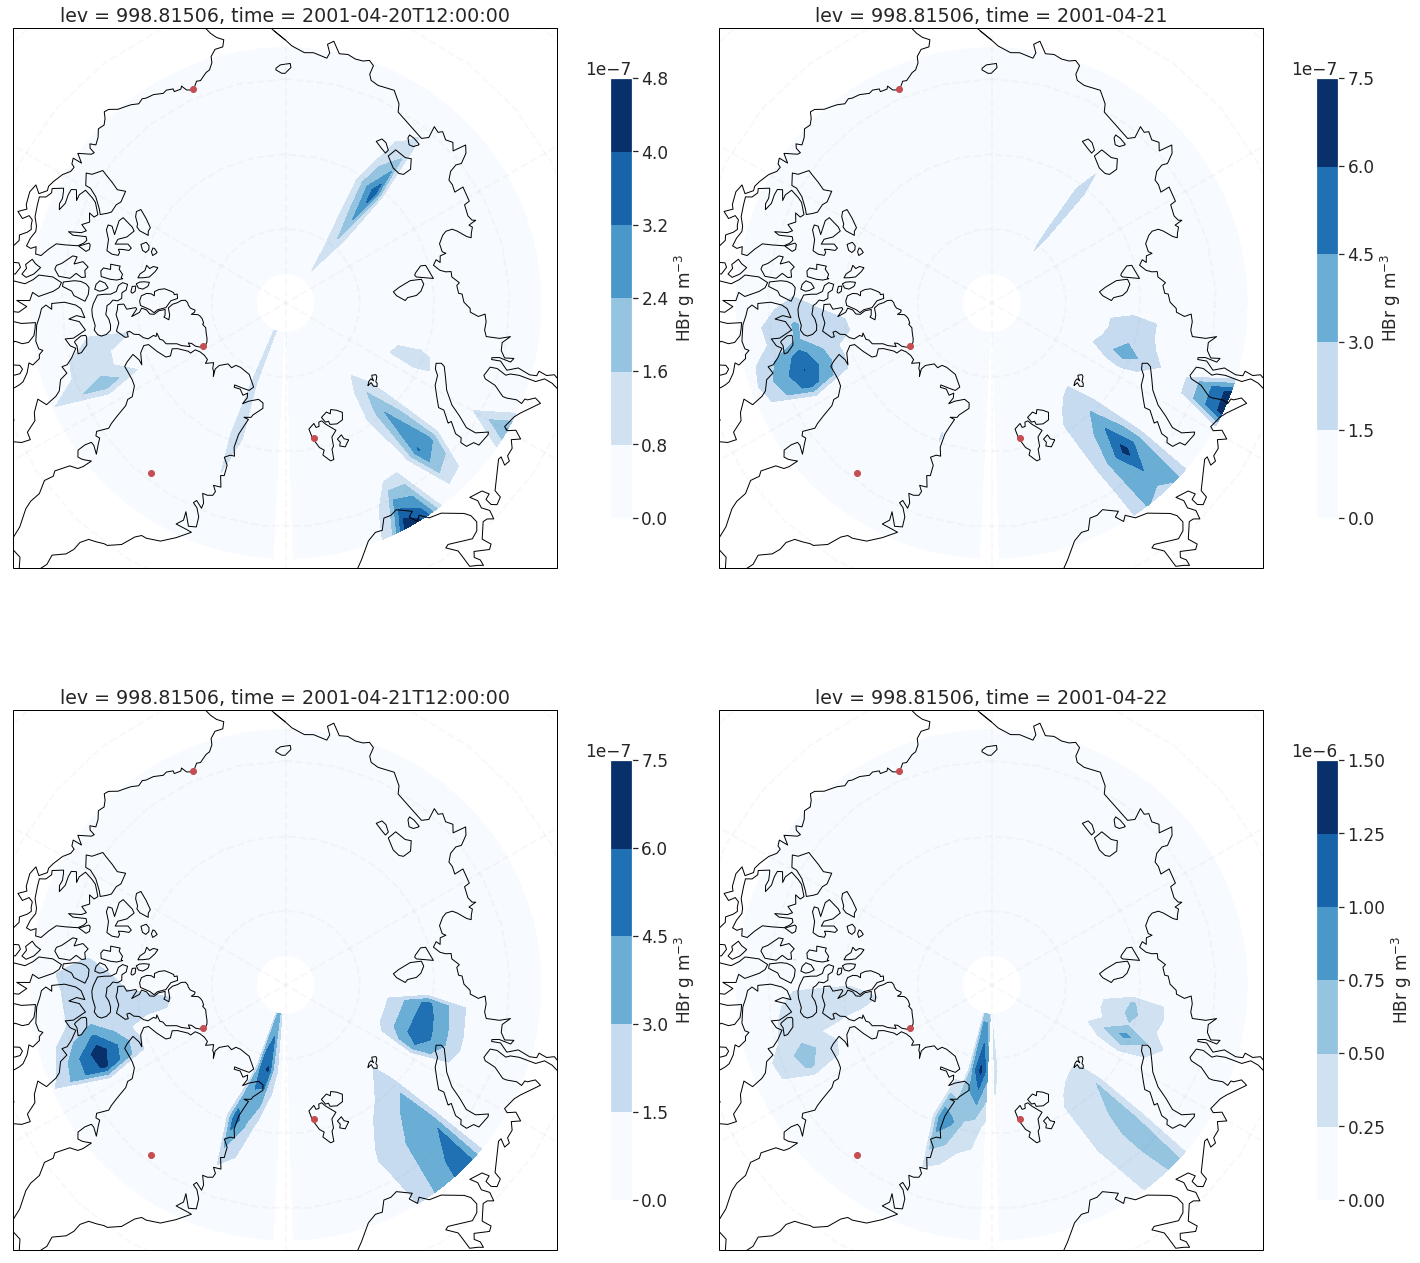
\includegraphics[width=\linewidth]{Chapter6_Results/images/polarHBr_newRestart.png}
    \caption{Concentration ($g m^{-3}$) of \chem{HBr} in the first model layer the Arctic at 12:00 and 00:00 (UTC) of the 20th, 21st and 22nd of April, 2001. The result is from Branch \ref{def:BE_PD_noCl} initialized with a new restart file with a \chem{HBr} concentration of 10 ppt. The red dots are the positions of the stations with observations in 2001 (see the map in Figure \ref{fig:stns} for reference)}
    \label{fig:polarHBr_newRestart}
\end{figure}

\begin{figure}[h]
    \centering
    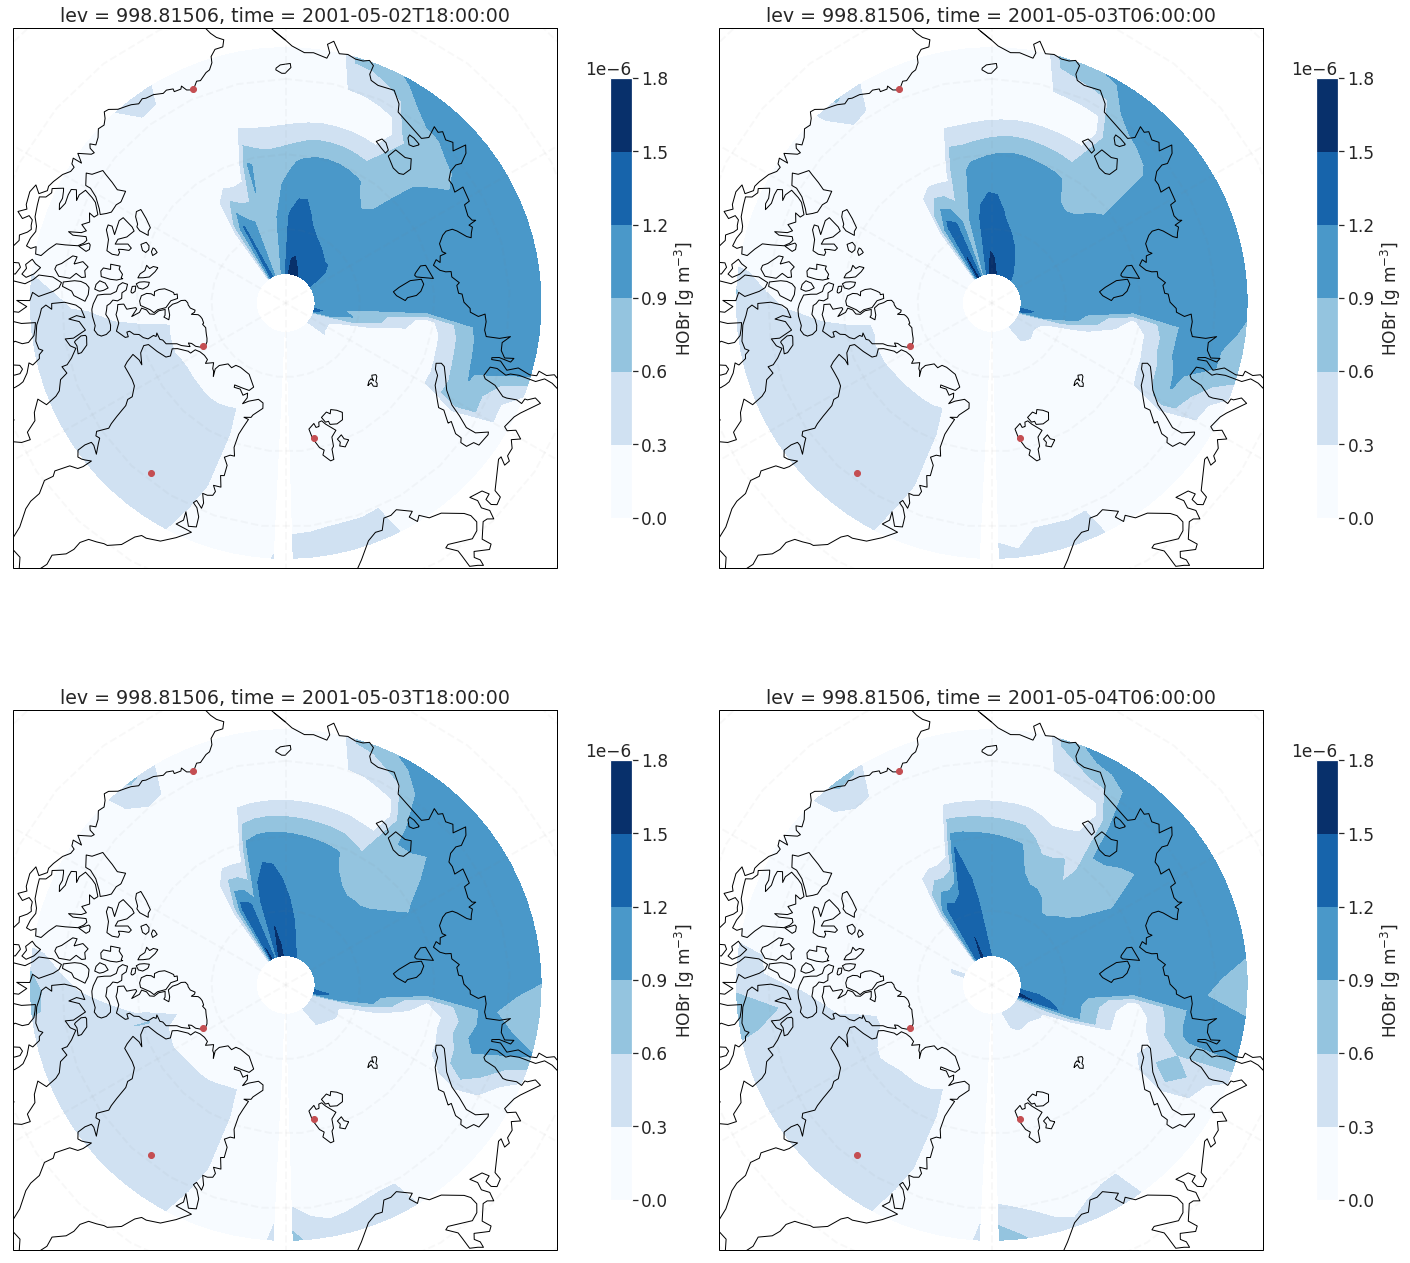
\includegraphics[width=\linewidth]{Chapter6_Results/images/polarHOBr_newRestart.png}
    \caption{Concentration ($g m^{-3}$) of \chem{HOBr} in the first model layer the Arctic at 18:00 and 06:00 (UTC) of the 2nd, 3rd and 4th of May, 2001. The result is from Branch \ref{def:BE_PD_noCl} initialized with a new restart file with a \chem{HBr} concentration of 10 ppt. The red dots are the positions of the stations with observations in 2001 (see the map in Figure \ref{fig:stns} for reference)}
    \label{fig:polarHOBr_newRestart}
\end{figure}

\medskip

The polar \chem{BrO}-column depicted in Figure \ref{fig:polarBro_newRestart} shows a \acrshort{vcd} on the order of $10^7 \text{molecules }$ cm$^{-2}$. 

\clearpage
\begin{figure}[h]
    \centering
    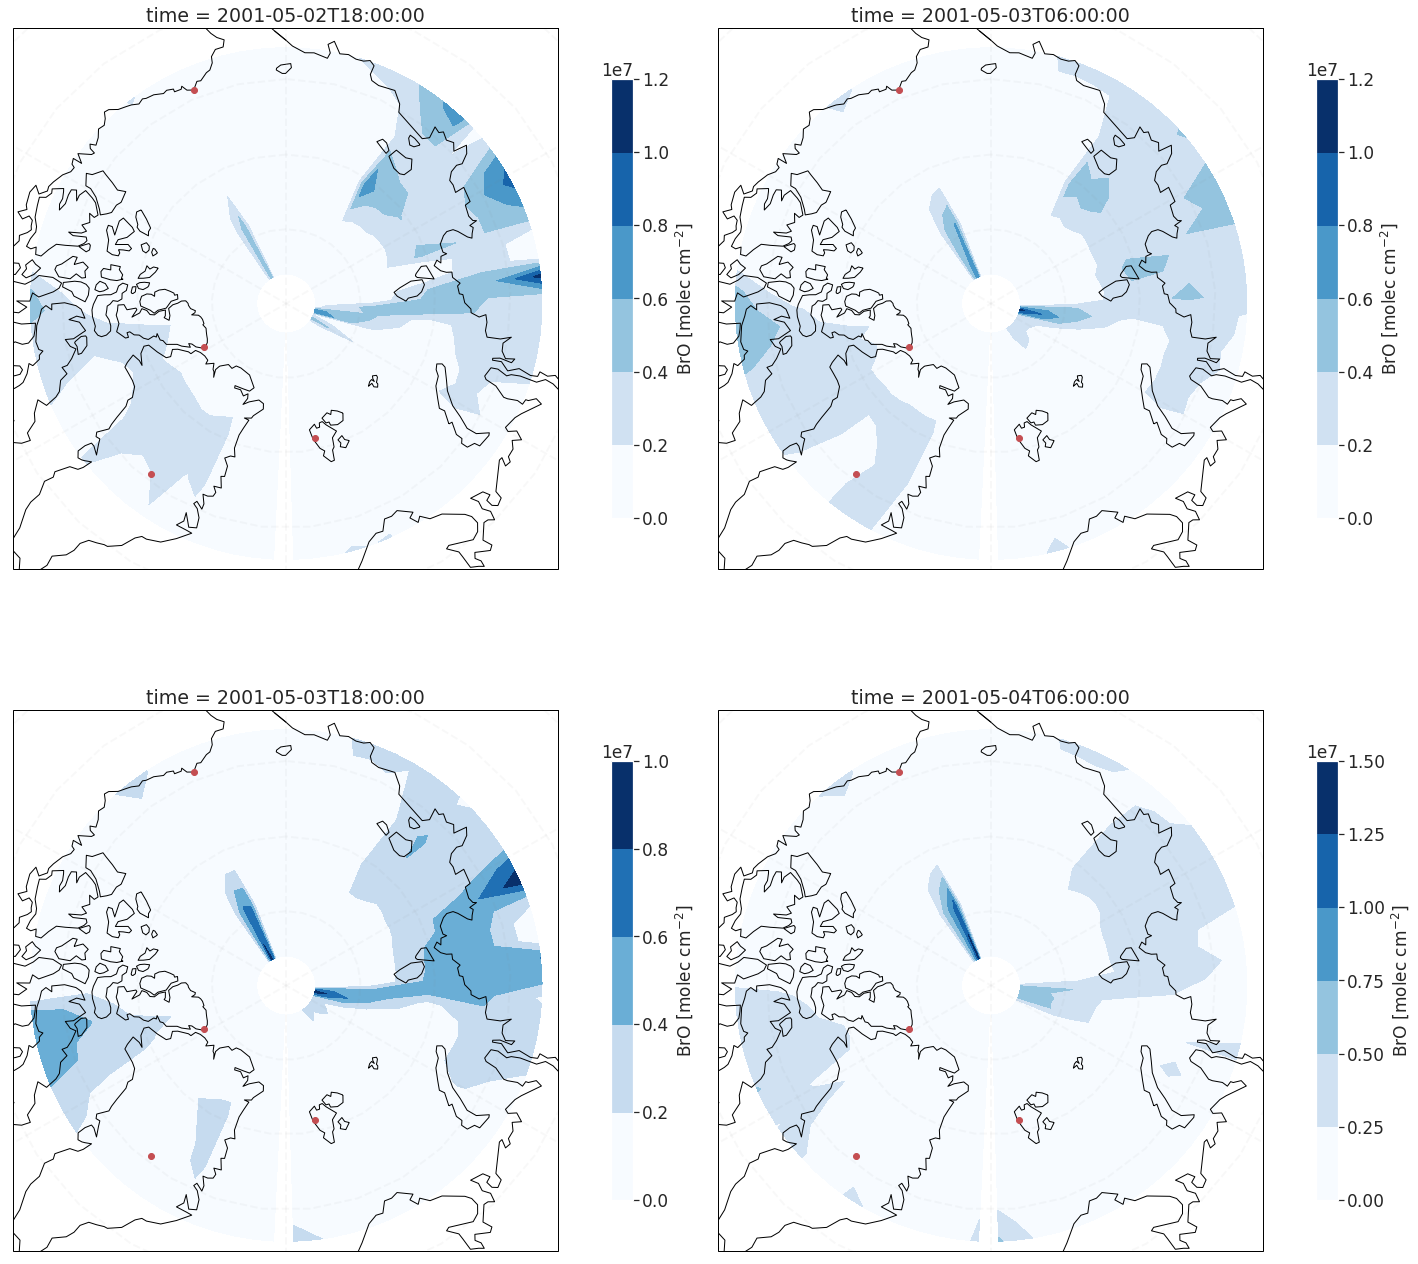
\includegraphics[width=\linewidth]{Chapter6_Results/images/polarBro_newRestart.png}
    \caption{Vertical column density ($molecules cm^{-2}$) of \chem{BrO} in the lowermost $\sim 250 m$ at 18:00 and 06:00 (UTC) on the  2nd, 3rd and 4th of May, 2001. The result is from Branch \ref{def:BE_PD_noCl} initialized with a new restart file with a \chem{HBr} concentration of 10 ppt. The red dots are the positions of the stations with observations in 2001 (see the map in Figure \ref{fig:stns} for reference)}
    \label{fig:polarBro_newRestart}
\end{figure}

\clearpage
\subsubsection{Hard-Coding Photodissociation and Adjusting the Henry'Law Coefficient}\label{sec:res_step3}

Figure \ref{fig:ozone_2001_step3} contains the modelled results from four new tests, whereas the original CTM3-run and the New Restart run was maintained from the previous section. Firstly, the Hard-coded P test was performed by hard-coding the photodissociation rates in \texttt{pchemc\_ij.f90}. In addition to this, two reactions were added in an attempt to better cycle the \chem{HOBr} and \chem{HBr} to avoid the anti-correlation seen in Figures \ref{fig:polarHBr_newRestart}-\ref{fig:polarHOBr_newRestart}:  

\begin{reaction}
    \chem{Br_2} + \chem{OH} \rightarrow \chem{HOBr} + \chem{Br}
    \label{rqn:oh_br2}
\end{reaction}


\begin{reaction}
    \chem{HBr} + \chem{OH} \rightarrow \chem{H_2O} + \chem{Br}
    \label{rqn:oh_hbr}
\end{reaction}

The hard-coded photodissociation rates had not previously calculated for Reactions \ref{R:18}, \ref{R:20} and \ref{R:12}. These were previously set to be solved by the fast-JX method (see Section \ref{sec:CTM3_photochemistry}), but did not work. Thus, these were hard-coded as was done previously (by \cite{Susanne}) for Reactions \ref{R:19} and \ref{R:1}. The photodissociation rates were then set to: 

\begin{itemize}
    \item $3\times10^{-4}$ s$^{-1}$ for Reaction \ref{R:18} (value from \cite{CAO})
    \item $0.014$ s$^{-1}$ for Reaction \ref{R:20}(value from \cite{CAO})
    \item $0.05\times10^{-8}$ s$^{-1}$ for Reaction \ref{R:12} (value from \cite{Papanastasiou2013}, Arctic spring dissociation rate, Figure 2, p. 3022)
\end{itemize}


%Testen viser bedring, men \chem{HBr} er fortsatt altfor høy- for treig våtavsetning? 

In the subsequent tests, the hard-coded photodissociation rates were included. These were concerning the Henry-coefficient (see Section \ref{sec:wet_dep_henrys_law}) which was initially implemented with the wrong units. The New H - low test was performed with: 


\begin{itemize}
    \item \chem{HBr}: $7.2\cdot 10^{-1} [M/amt]$, $6100 K$ (Taken from: \cite{Chameides1992})
    \item \chem{HCl}: $1.9\cdot10^1 [M/atm]$, $600 K$ (Taken from: \cite{dean1999})
\end{itemize}

The New H- high test was performed with:  

\begin{itemize}
    \item \chem{HBr}: $2.5 \cdot 10^{1} [M/amt]$, $370 K$ (Taken from: \cite{dean1999})
    \item \chem{HCl}: $1.9\cdot10^1 [M/atm]$, $600 K$ (Taken from: \cite{dean1999})
\end{itemize}

Finally, the latter was tested with a higher resolution (HTWO). 

\medskip

Figure \ref{fig:ozone_2001_step3} shows that the new tests ozone produce a lower mixing ratio than both the original CTM3 and the New Restart-test from the previous section. They also produce lower ozone concentrations at the stations compared to measurements. 

%Fin ODE klokka 21 den 29/3! Høye Br og BrO og lav ozon! (fil 88) 


\begin{figure}[ht]
    \centering
    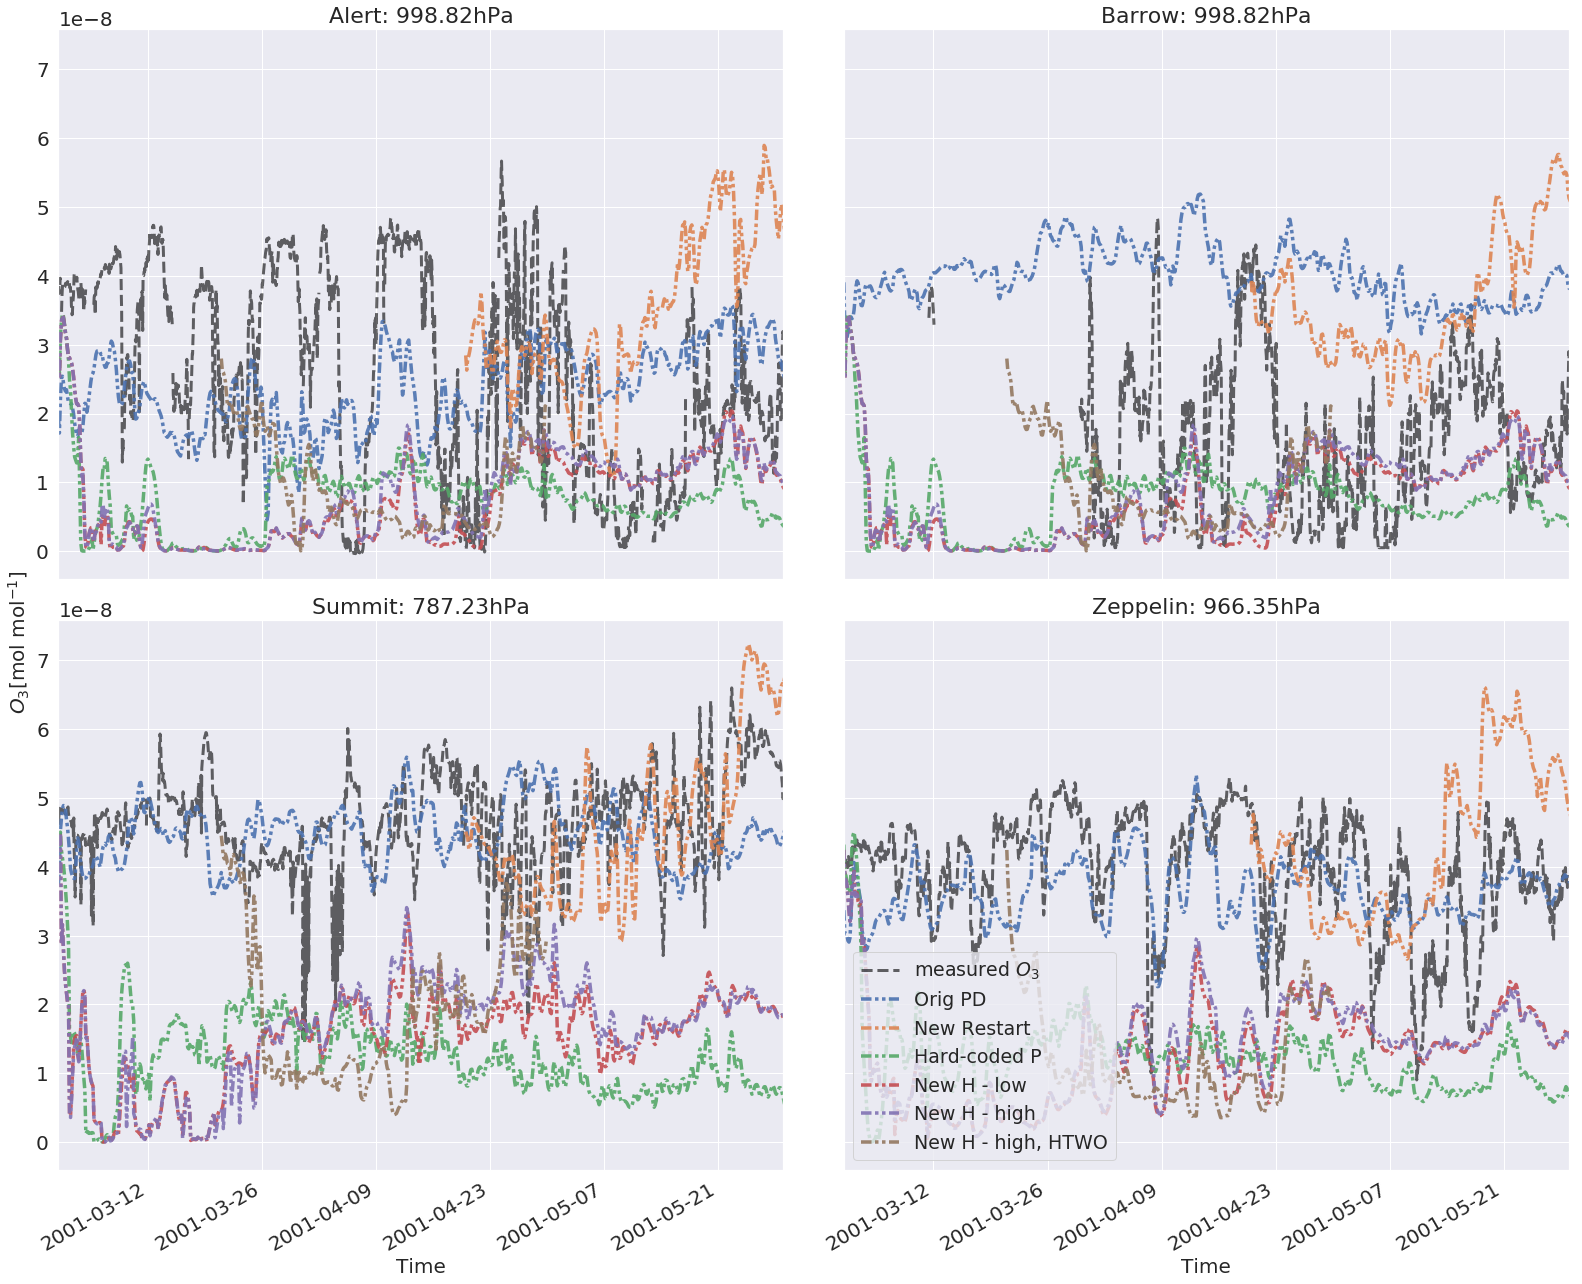
\includegraphics[width=\linewidth]{Chapter6_Results/images/ozone_2001_step3.png}
    \caption{Ozone measurements (black line) and model results from the original CTM3 (blue line) (these two are the same as in Figure \ref{fig:CompObsOrigBE}), test with new restart file from Section \ref{sec:res_step2} (turquoise line), hard-coded photodissociation rates (green line), new (low) Henry's law constant of $7.2\times10^{-1} M atm ^{-1}$ and $6100 K$ (light green line), new (high) Henry's law constant of $2.5\times10^{1} M atm ^{-1}$ and $370 K$ (yellow line) and the latter ran at \texttt{HTWO} resolution (orange line) at the four different stations, Alert (top left), Barrow (top right), Summit (lower left) and Zeppelin (lower right) with available measurements in 2001. Model results were taken from the approximate altitude of the station in hPa. PD = present day, P = photolysis rate, H = Henry's Law}
    \label{fig:ozone_2001_step3}
\end{figure}

\medskip

Figure \ref{fig:vertHBr_HTWO_step3} contains the vertical column of the \chem{HBr} mixing ratio at \texttt{HTWO} resolution. The mixing ratio remains around $3\times10^{-10}$ mol mol$^{-1}$ (300 ppt) for both the tests. Likewise, Figure \ref{fig:polarHBr_HTWO_step3} contains concentrations of \chem{HBr} on the order of $6\times10^{-6} $g m$^{-3}$. The concentration of \chem{HOBr} is shown in Figure \ref{fig:polarHOBr_HTWO_step3}. The same anti-correlation is shown between \chem{HBr} and \chem{HOBr} as in the previous section. 

%\begin{figure}[h]
    \centering
    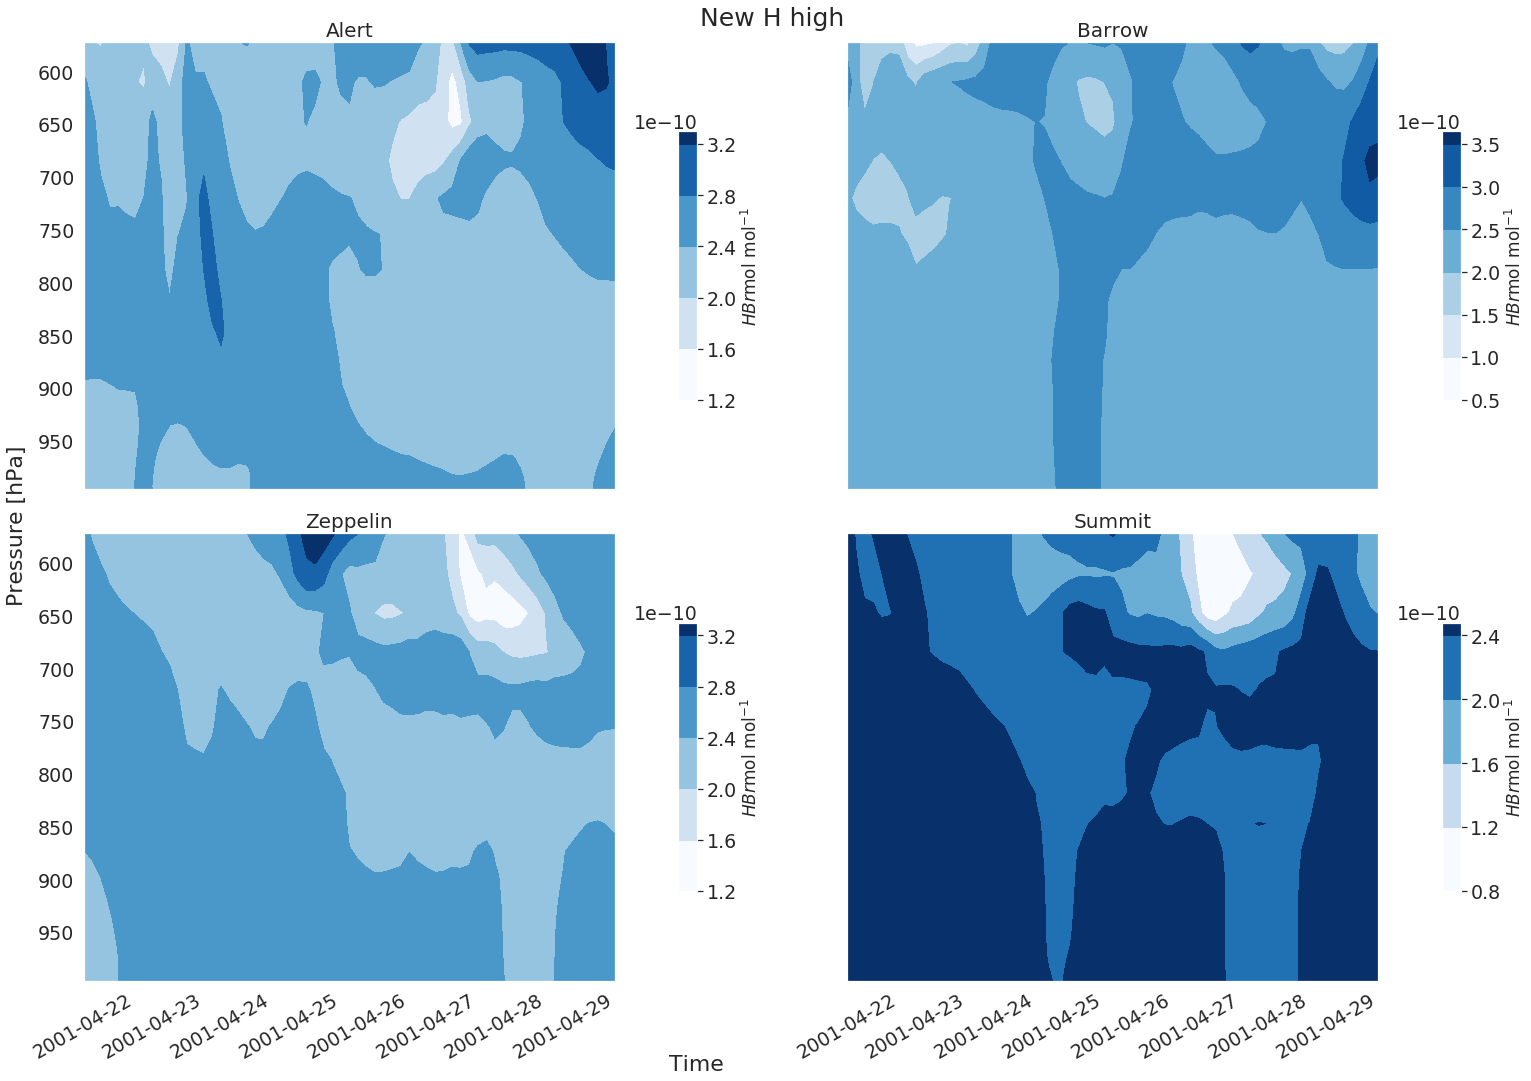
\includegraphics[width=\linewidth]{Chapter6_Results/images/vertHBr_HFOUR_step3.png}
    \caption{Mixing ratio ($mol mol^{-1}$) of \chem{HBr} in the model layers up to $\sim 600 hPa$ at the four different stations Alert (top left), Barrow (top right), Zeppelin (lower left) and Summit (lower right) in April, 2001. The result is from the test including hard-coded photodissociation rates as well as a new (high) Henry-coefficient at HFOUR resolution}
    \label{fig:vertHBr_HFOUR_step3}
\end{figure}
\begin{figure}[h]
    \centering
    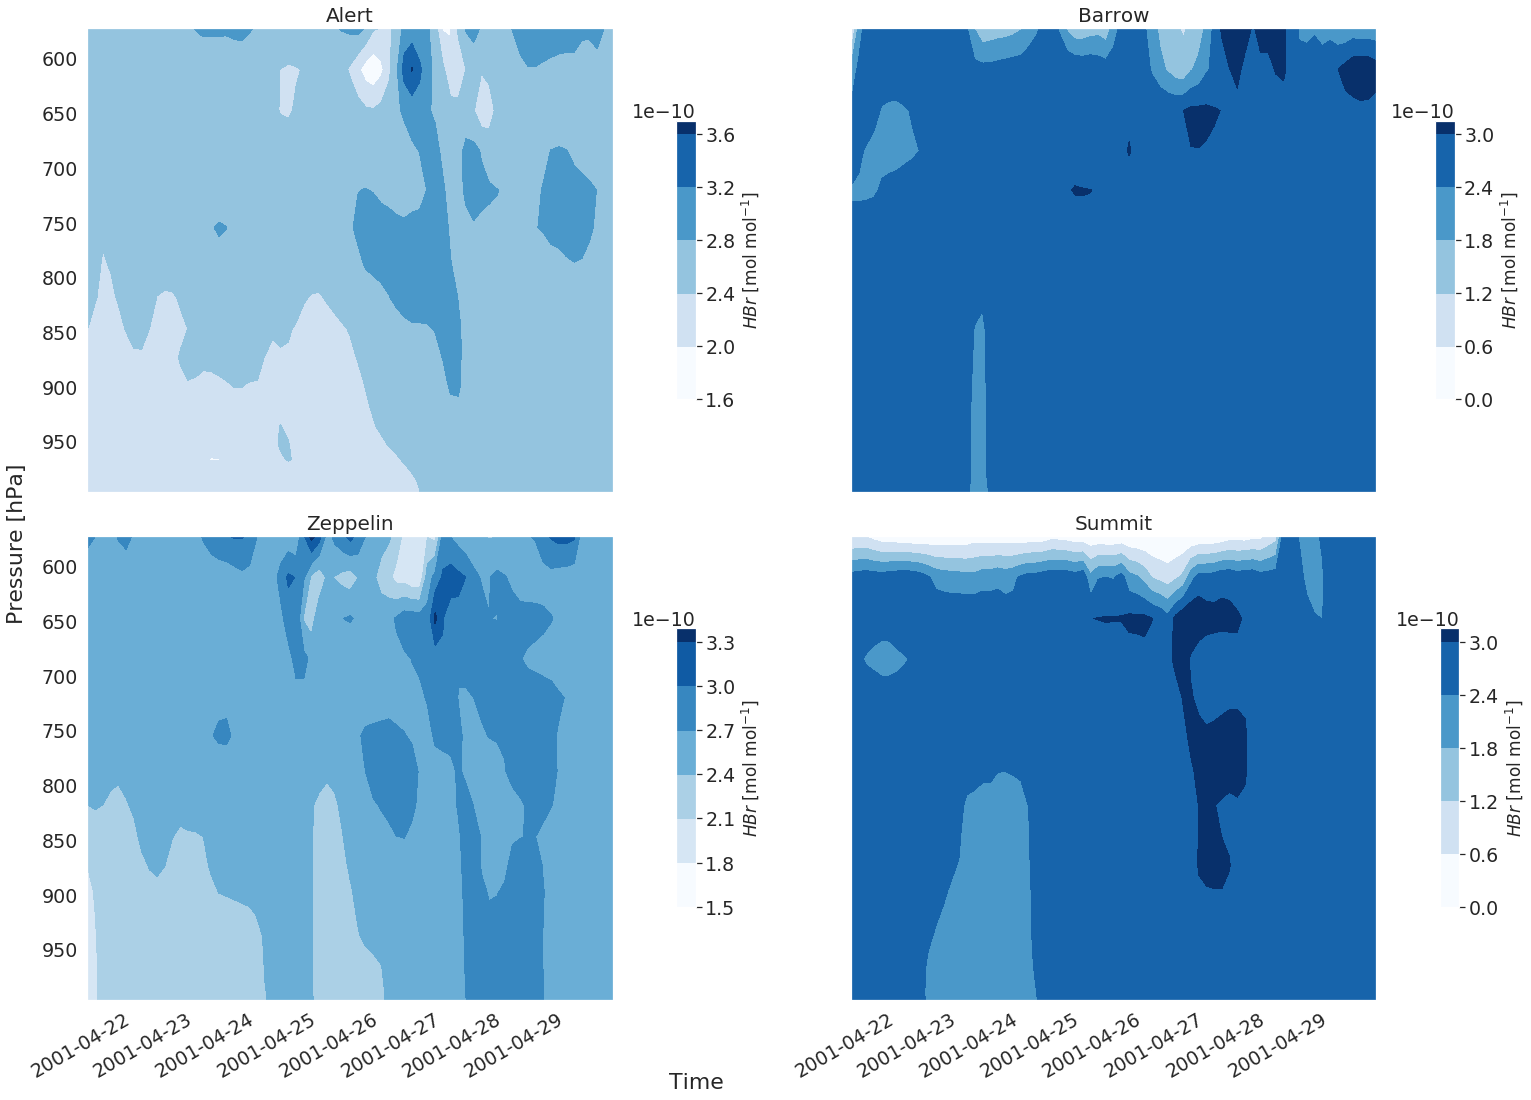
\includegraphics[width=\linewidth]{Chapter6_Results/images/vertHBr_HTWO_step3.png}
    \caption{Mixing ratio ($mol mol^{-1}$) of \chem{HBr} in the model layers up to $\sim 600 hPa$ at the four different stations Alert (top left), Barrow (top right), Zeppelin (lower left) and Summit (lower right) in April, 2001. The result is from the test including hard-coded photodissociation rates as well as a new (high) Henry-coefficient at HTWO resolution}
    \label{fig:vertHBr_HTWO_step3}
\end{figure}

%\begin{figure}[h]
    \centering
    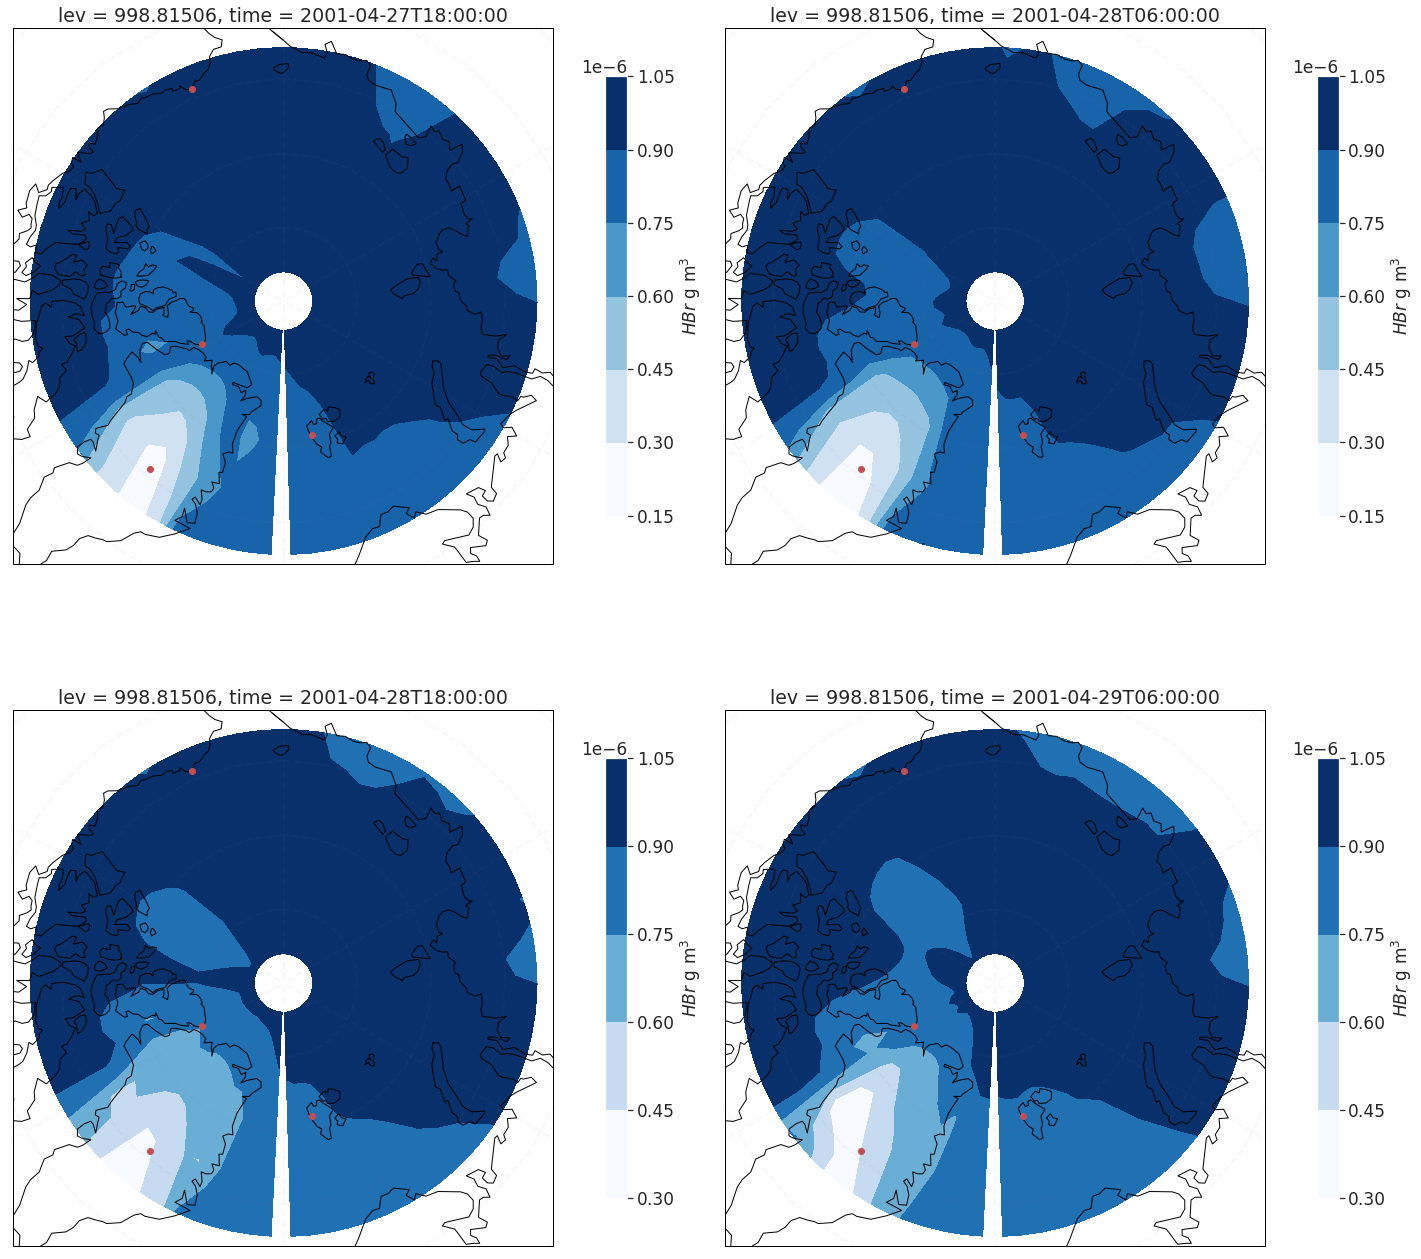
\includegraphics[width=\linewidth]{Chapter6_Results/images/polarHBr_HFOUR_step3.png}
    \caption{Concentration ($g m^{-3}$) of \chem{HBr} in the first model layer the Arctic at 18:00 and 06:00 (UTC) of the 27th, 28th and 29th of April, 2001. The result is from the test including hard-coded photodissociation rates as well as a new (high) Henry-coefficient at HFOUR resolution. The red dots are the positions of the stations with observations in 2001 (see the map in Figure \ref{fig:stns} for reference)}
    \label{fig:polarHBr_HFOUR_step3}
\end{figure}
\begin{figure}[h]
    \centering
    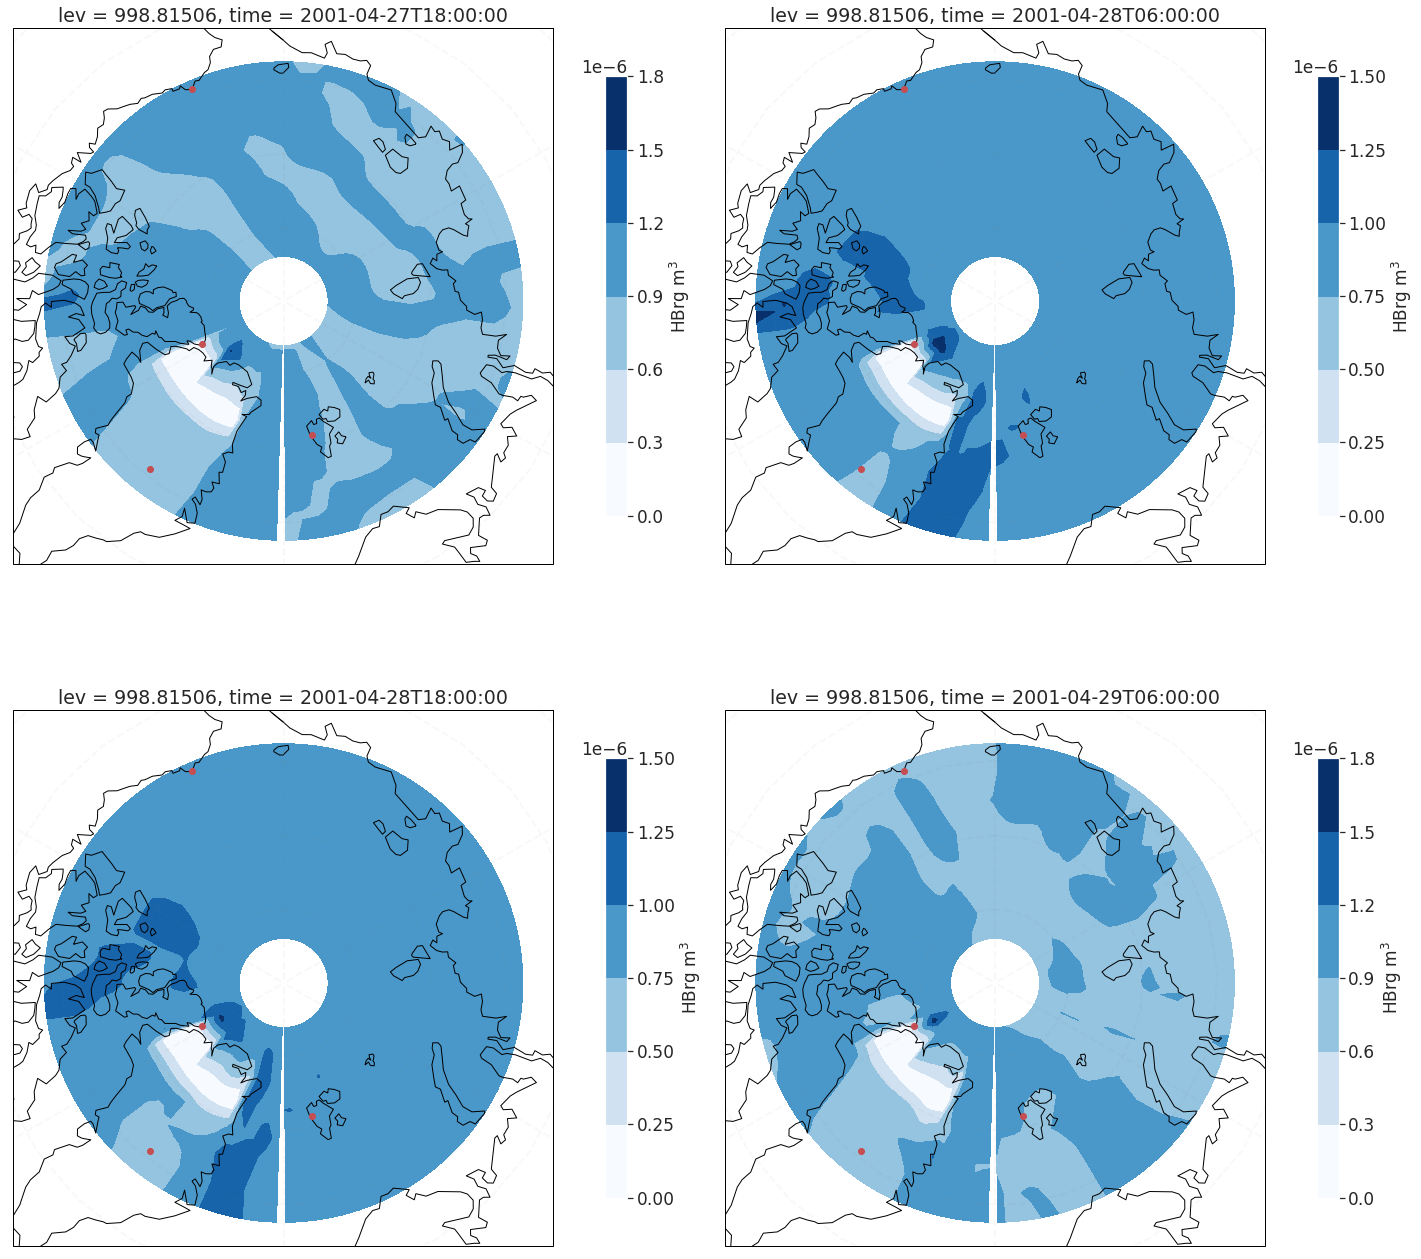
\includegraphics[width=\linewidth]{Chapter6_Results/images/polarHBr_HTWO_step3.png}
    \caption{Concentration ($g m^{-3}$) of \chem{HBr} in the first model layer the Arctic at 18:00 and 06:00 (UTC) of the 27th, 28th and 29th of April, 2001. The result is from Branch \ref{def:BE_PD_noCl} including hard-coded photodissociation rates as well as a new (high) Henry-coefficient at HTWO resolution. The red dots are the positions of the stations with observations in 2001 (see the map in Figure \ref{fig:stns} for reference)}
    \label{fig:polarHBr_HTWO_step3}
\end{figure}

\begin{figure}[h]
    \centering
    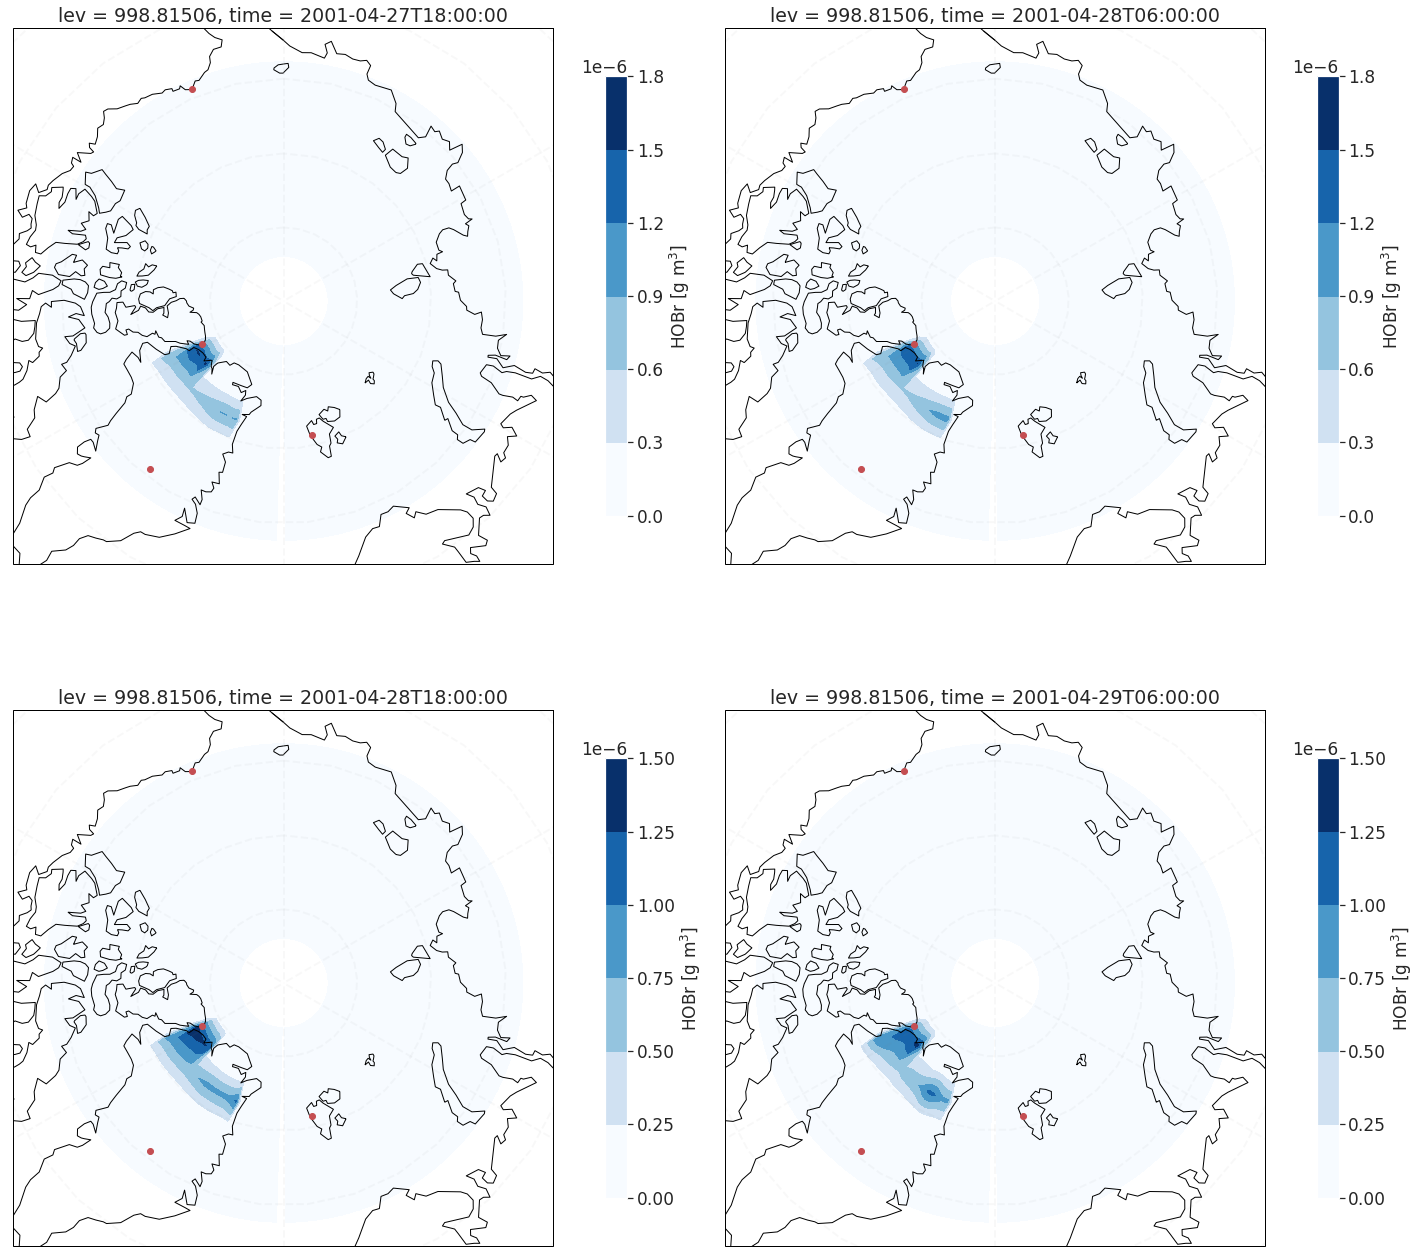
\includegraphics[width=\linewidth]{Chapter6_Results/images/polarHOBr_HTWO_step3.png}
    \caption{Concentration ($g m^{-3}$) of \chem{HOBr} in the first model layer the Arctic at 18:00 and 06:00 (UTC) of the 27th, 28th and 29th of April, 2001. The result is from  Branch \ref{def:BE_PD_noCl} including hard-coded photodissociation rates as well as a new (high) Henry-coefficient at HTWO resolution. The red dots are the positions of the stations with observations in 2001 (see the map in Figure \ref{fig:stns} for reference)}
    \label{fig:polarHOBr_HTWO_step3}
\end{figure}


\medskip

The \chem{BrO} \acrshort{vcd} is shown in Figure \ref{fig:polarBrO_HTWO_step3}. The  \acrshort{vcd} now has a maximum of about $3\times10^8$ molecules cm$^{-2}$. 

%\begin{figure}[h]
    \centering
    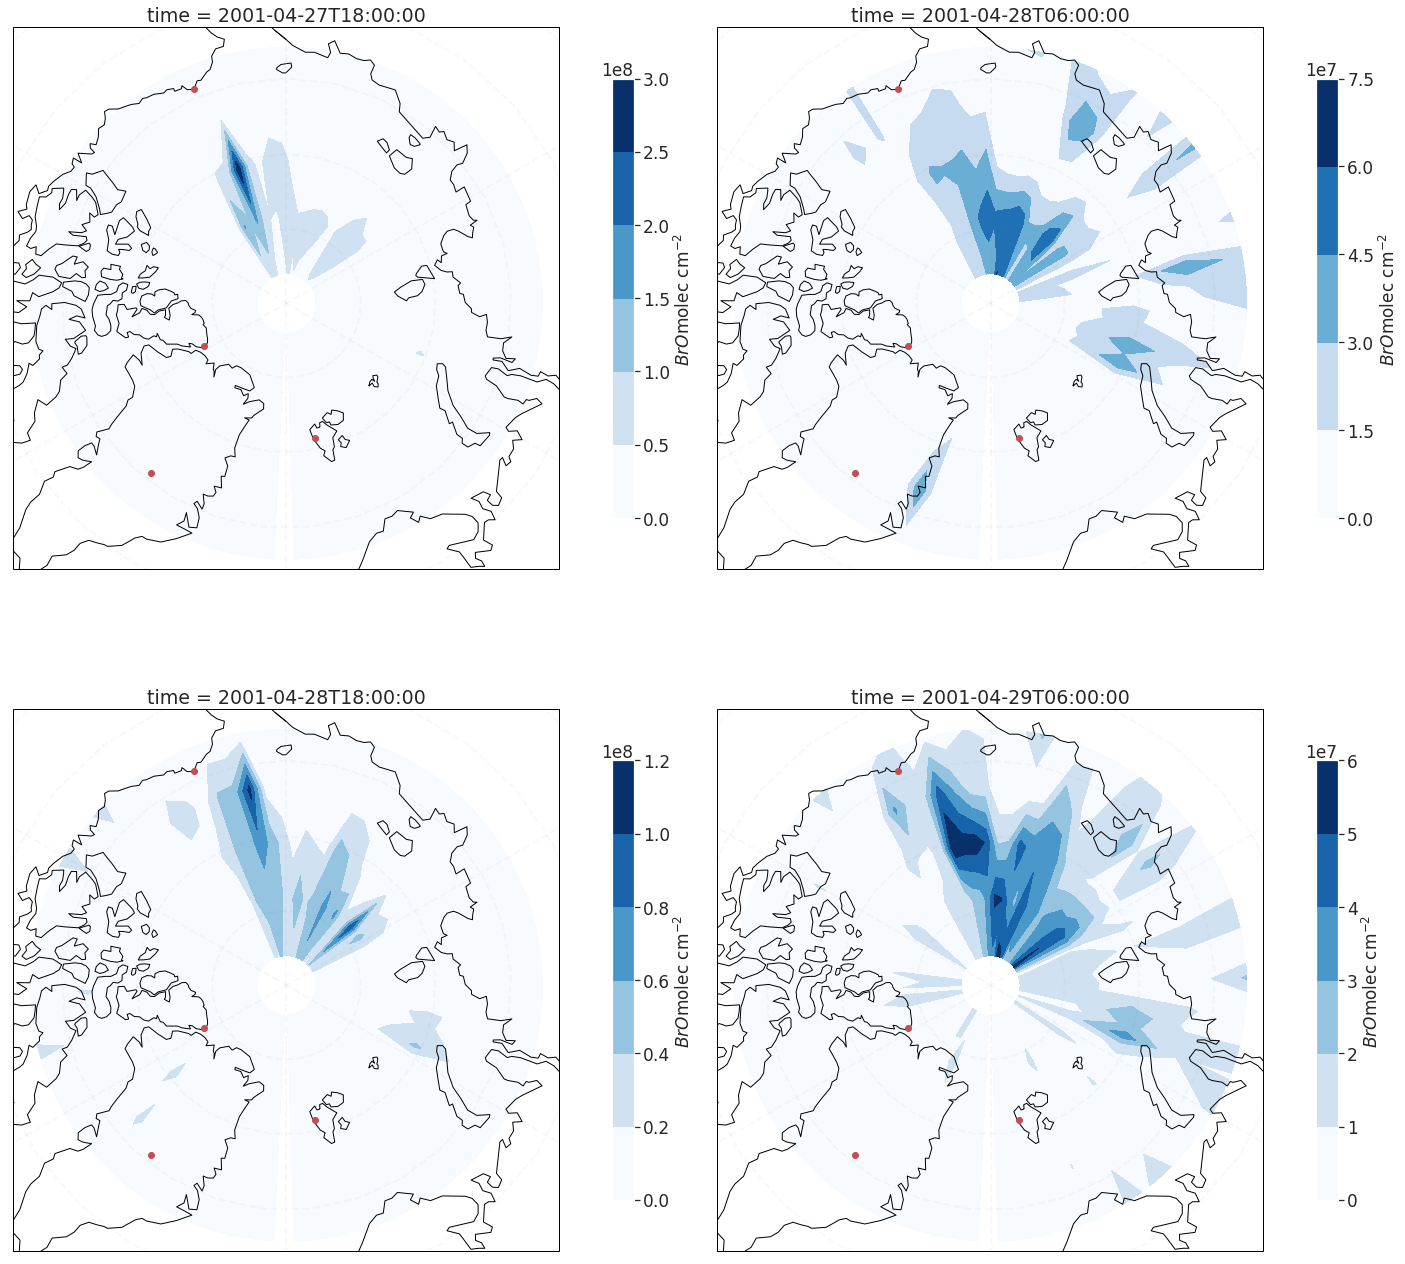
\includegraphics[width=\linewidth]{Chapter6_Results/images/polarBrO_HFOUR_step3.png}
    \caption{Vertical column density ($molecules cm^{-2}$) of \chem{BrO} in the lowermost $\sim 250 m$ at 18:00 and 06:00 (UTC) of the 27th, 28th and 29th of April, 2001. The result is from the test including hard-coded photodissociation rates as well as a new (high) Henry-coefficient at HFOUR resolution. The red dots are the positions of the stations with observations in 2001 (see the map in Figure \ref{fig:stns} for reference)}
    \label{fig:polarBrO_HFOUR_step3}
\end{figure}
\begin{figure}[h]
    \centering
    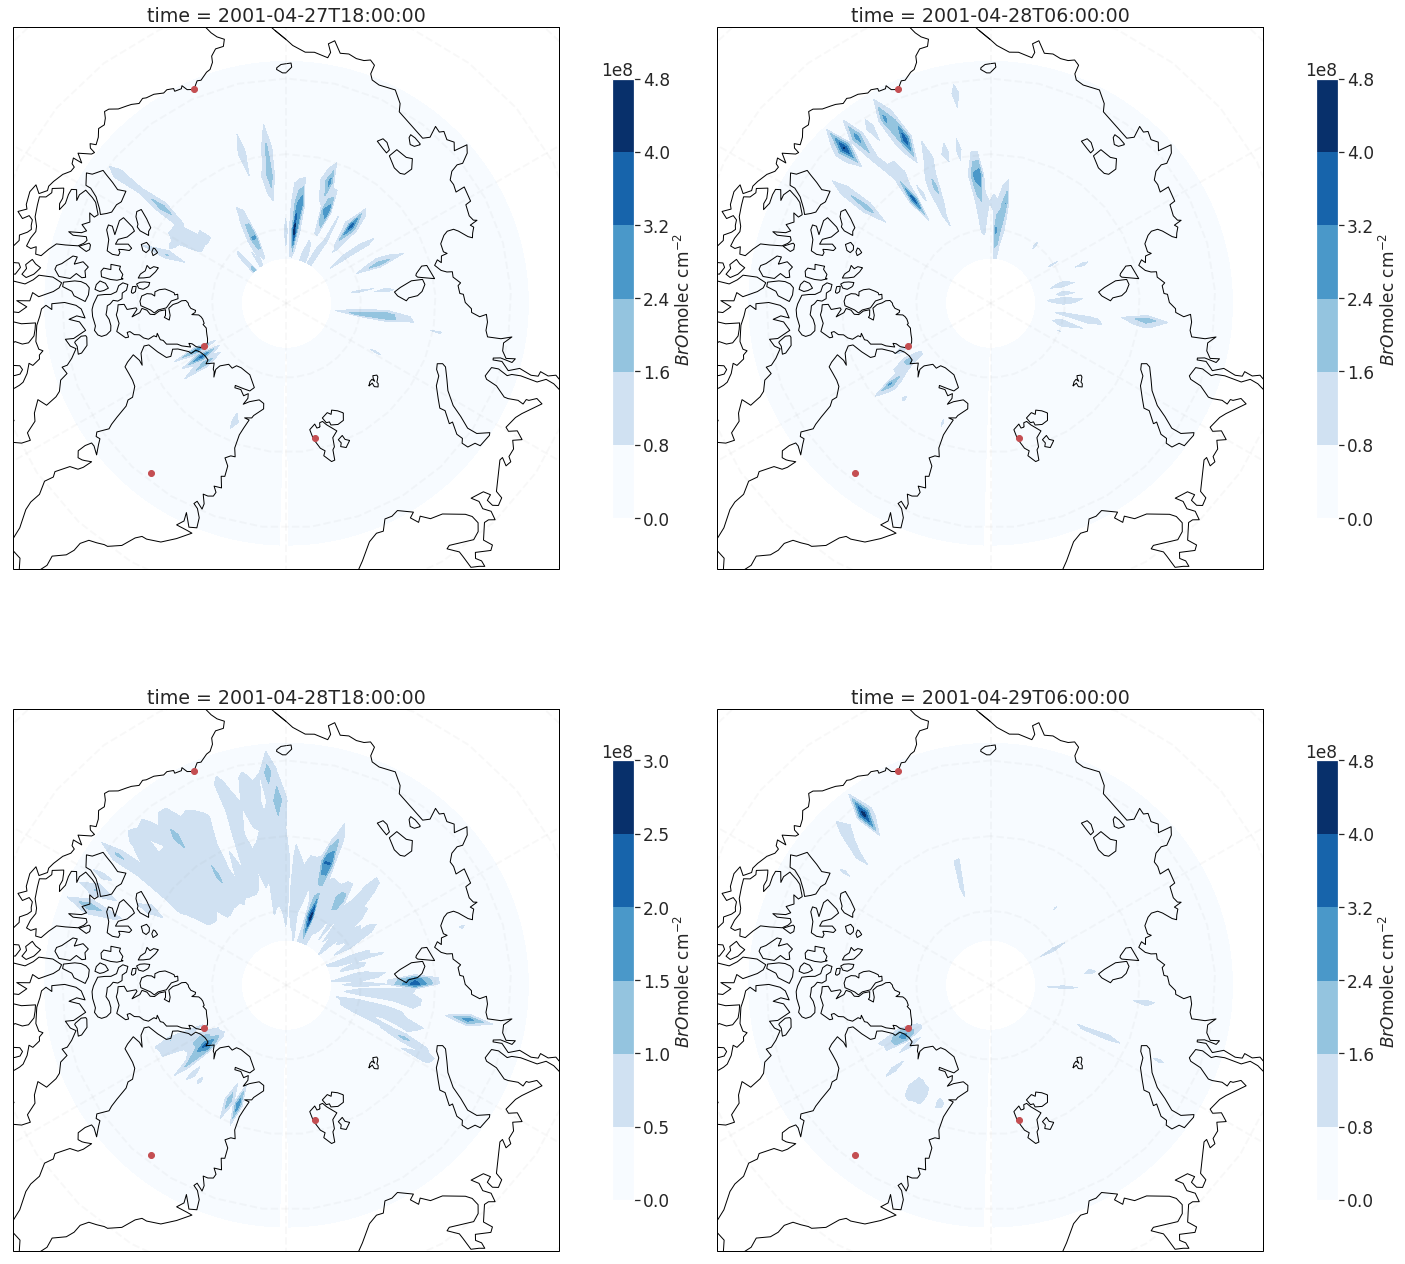
\includegraphics[width=\linewidth]{Chapter6_Results/images/polarBrO_HTWO_step3.png}
    \caption{Vertical column density ($molecules cm^{-2}$) of \chem{BrO} in the lowermost $\sim 250 m$ at 18:00 and 06:00 (UTC) of the 27th, 28th and 29th of April, 2001. The result is from  Branch \ref{def:BE_PD_noCl} including hard-coded photodissociation rates as well as a new (high) Henry-coefficient at HFOUR resolution. The red dots are the positions of the stations with observations in 2001 (see the map in Figure \ref{fig:stns} for reference)}
    \label{fig:polarBrO_HTWO_step3}
\end{figure}

\clearpage
\subsubsection{Changing Henry's law coefficient and photodissociation of \chem{HOBr}}\label{sec:res_step4}

Due to issues regarding making a final production run (i.e. running the CTM3 for 6 months) (the problems and discussion concerning this are outlined in the Discussion Section \ref{sec:disc_step4}), Branch \ref{def:BE_PD_noCl} was altered yet again with a new Henry's law constant for the wet deposition of \chem{HBr} taken from \cite{Sander99}: 

\begin{itemize}
    \item $1.3\times10^9/K_\text{A} [M/atm]$, $10 000 K$ (Taken from: \cite{Brimblecombe1988TheSA})
    \item The acid dissociation constant, $K_\text{A}$, was taken as $\ln{K_\text{A}} \approx 9.8$ (\cite{Levanov})
\end{itemize}

As well as a new photodissociation rate for \chem{HOBr}:

\begin{itemize}
    \item $3\times10^{-3}$ s$^{-1}$ for Reaction \ref{R:18} (based on value from \cite{CAO}, but an order of 10 faster)
\end{itemize}

This branch was initialized with the restart file provided from \cite{StefaniePersonal} (see Section \ref{subsec:restart_files}) and ran for 6 months runs at \texttt{HTWO} resolution. The resulting ozone mixing ratio at the four stations can be seen in Figure \ref{fig:ozone_2001_step4}. The black and blue line represents the measured ozone and the results from the original CTM3, respectively. The turquoise line represents the result maintained from the section above, which was ran at \texttt{HTWO}-resolution and was supposed to be the basis for the final production run. Finally, the green line represents the actual production run, in which the differences are explained above. The ozone concentration in the final version starts out lower than what was measured at the different stations, and lower than the other model runs. At the end of the period, the concentration in the final version increases. %Naturlig at det tar litt tid for at det skal stabilisere seg, fordi restartfila har helt forskjellig kjemi --> burde hatt en spin up både for HTWO og ny kjemi


\begin{figure}[ht]
    \centering
    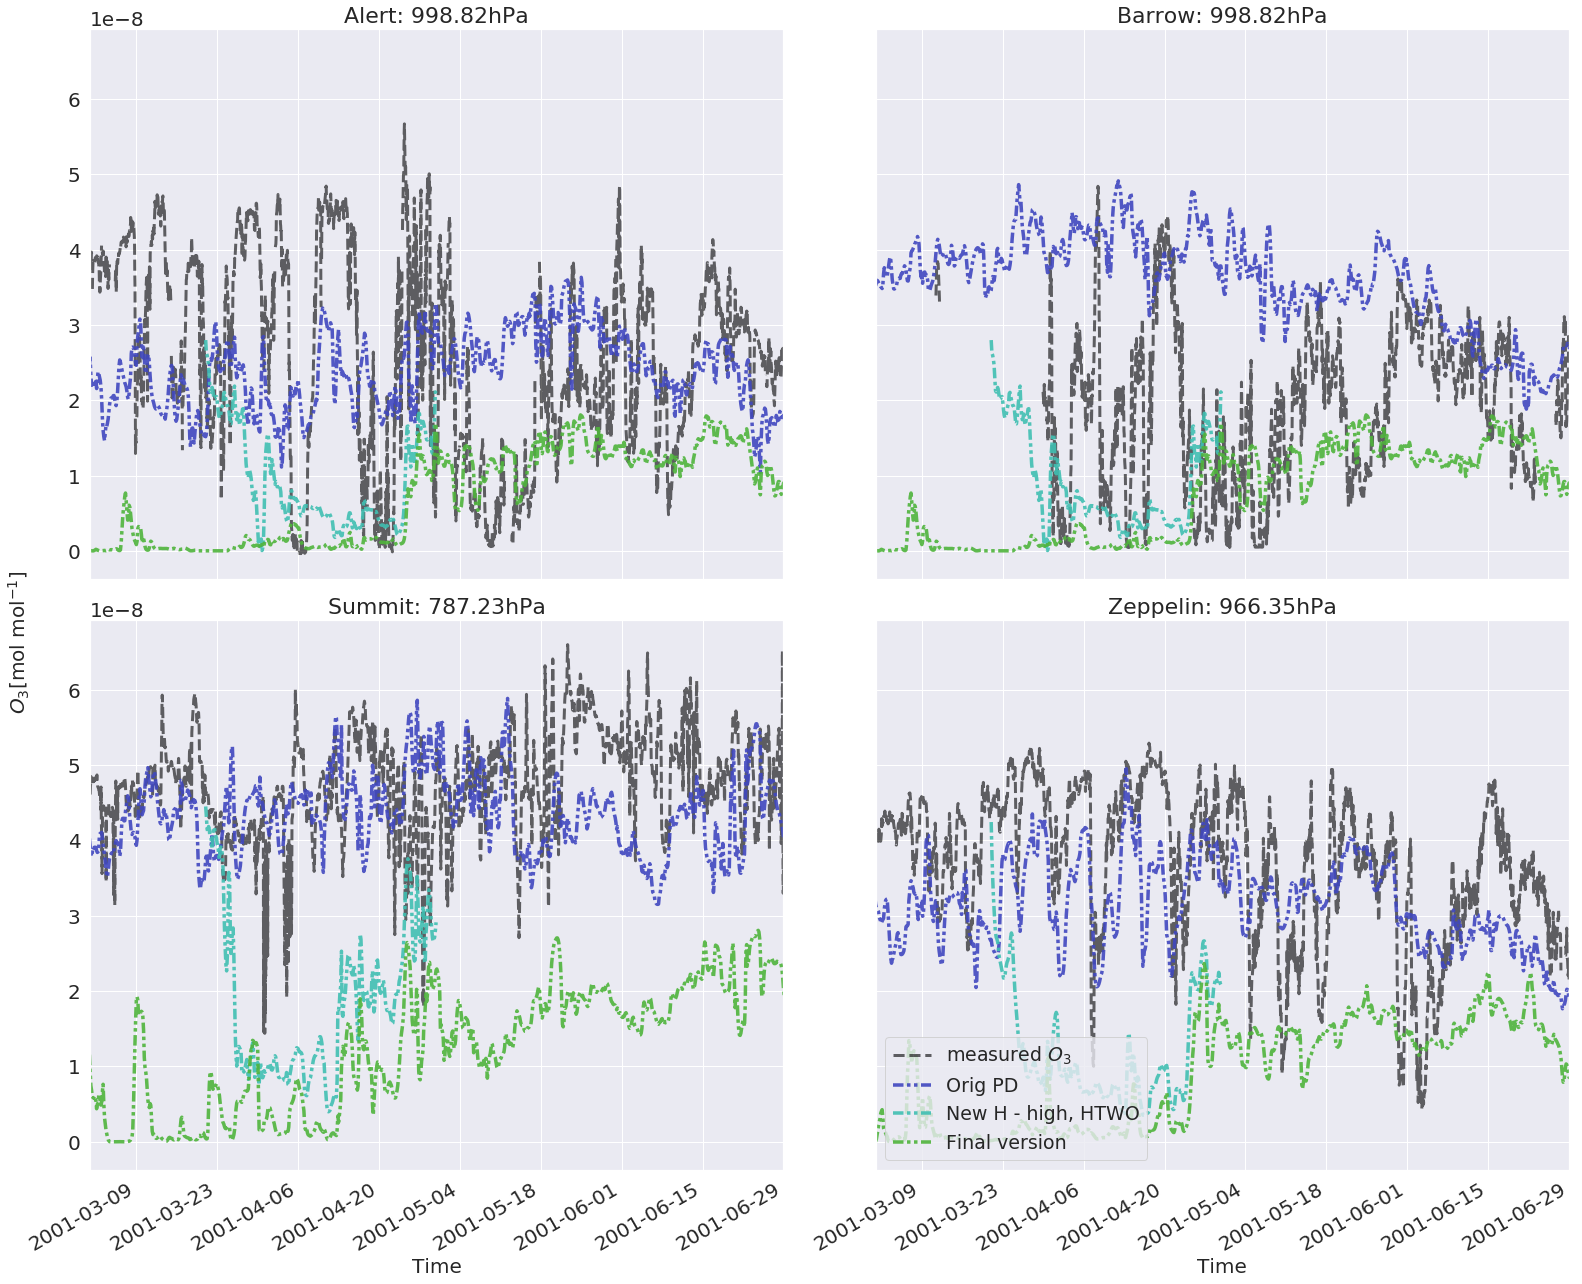
\includegraphics[width=\linewidth]{Chapter6_Results/images/ozone_2001_step4.png}
    \caption{Ozone measurements (black line) and model results from the original CTM3 (blue line) (these two are the same as in Figure \ref{fig:CompObsOrigBE}), Henry's law constant of $2.5\times10^{1} M atm ^{-1}$ and $370 K$ at \texttt{HTWO} resolution (turquoise line) and a final version with a new, higher Henry's law constant of $7.2\times10^{4} M atm ^{-1}$ and $10 000 K$ also at \texttt{HTWO} resolution (green line) at the four different stations, Alert (top left), Barrow (top right), Summit (lower left) and Zeppelin (lower right) with available measurements in 2001. Model results were taken from the approximate altitude of the station in hPa. PD = present day, P = photolysis rate, H = Henry's Law}
    \label{fig:ozone_2001_step4}
\end{figure}
\medskip

Figure \ref{fig:vertHBr_step4} contains the vertical profile of \chem{HBr} above the fours stations up to 600 hPa. The concentration is on the order of $10^{-11}$ mol/mol (10 ppt). The polar concentration in the first model layer is shown in Figure \ref{fig:polarHBr_step4}. The concentration is on the order of $10^{-7}$ gm$^{-3}$. 

\medskip


\begin{figure}[ht]
    \centering
    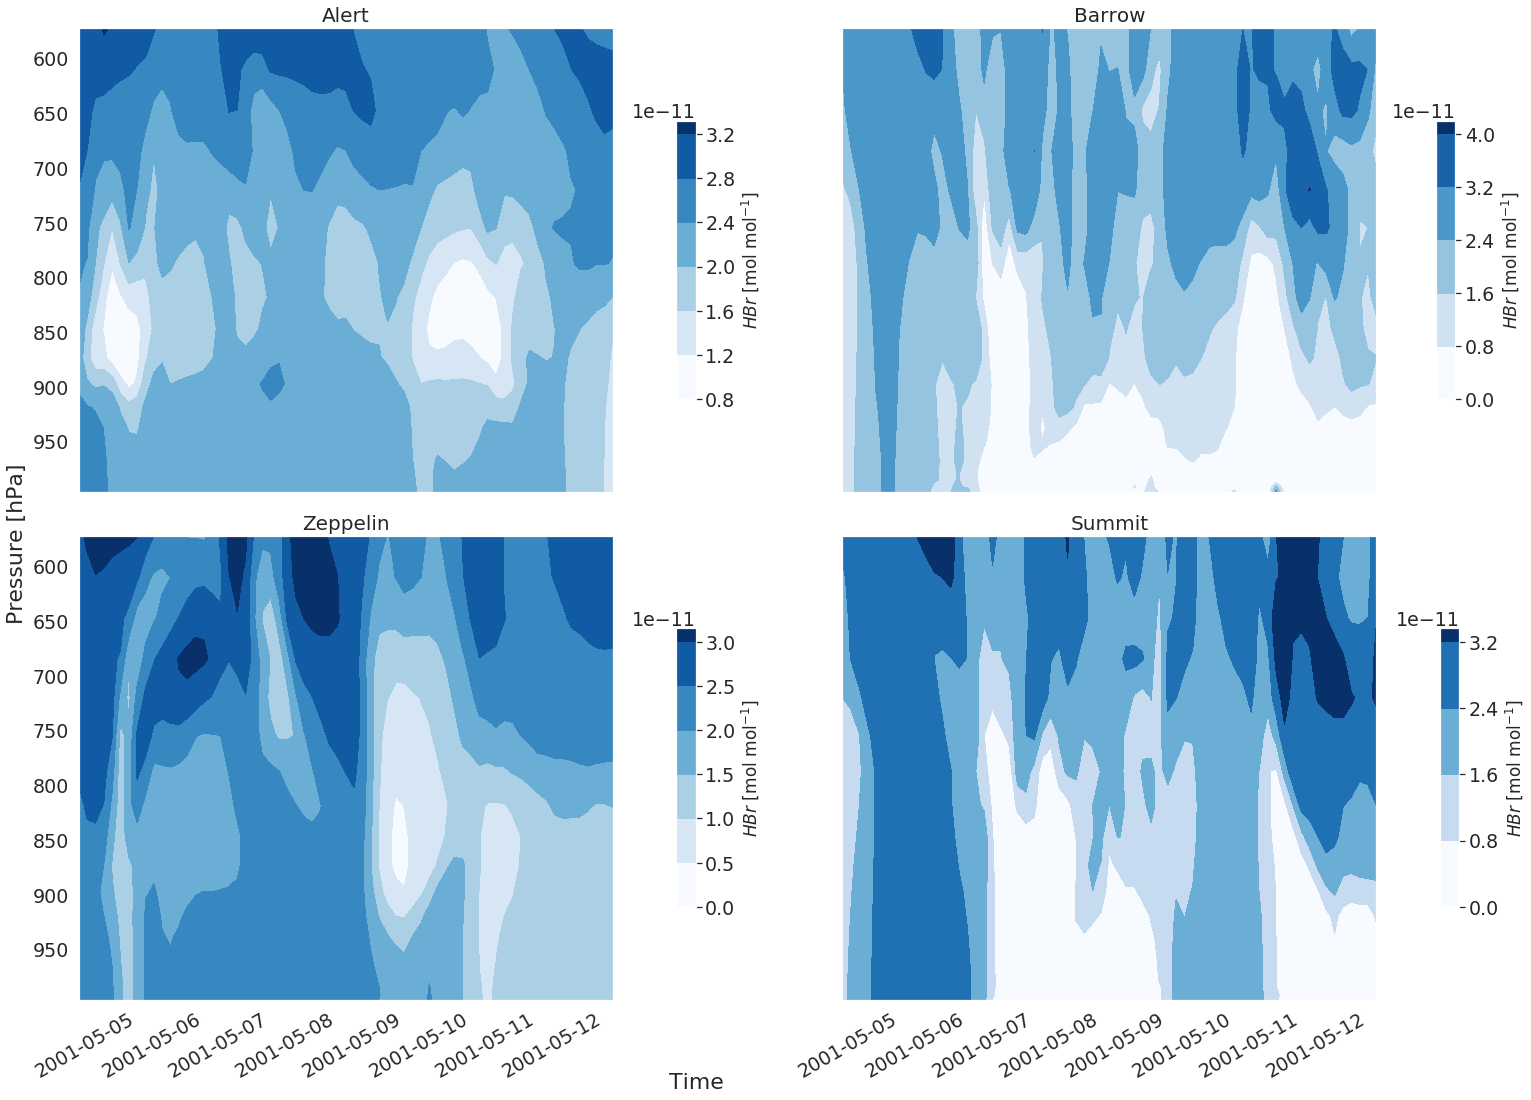
\includegraphics[width = \linewidth]{Chapter6_Results/images/vertHBr_step4.png}
    \caption{Mixing ratio ($mol mol^{-1}$) of \chem{HBr} in the model layers up to $\sim 600 hPa$ at the four different stations Alert (top left), Barrow (top right), Zeppelin (lower left) and Summit (lower right) in April-May, 2001. The results are from the final version of the CTM3}
    \label{fig:vertHBr_step4}
\end{figure}
\begin{figure}[h]
    \centering
    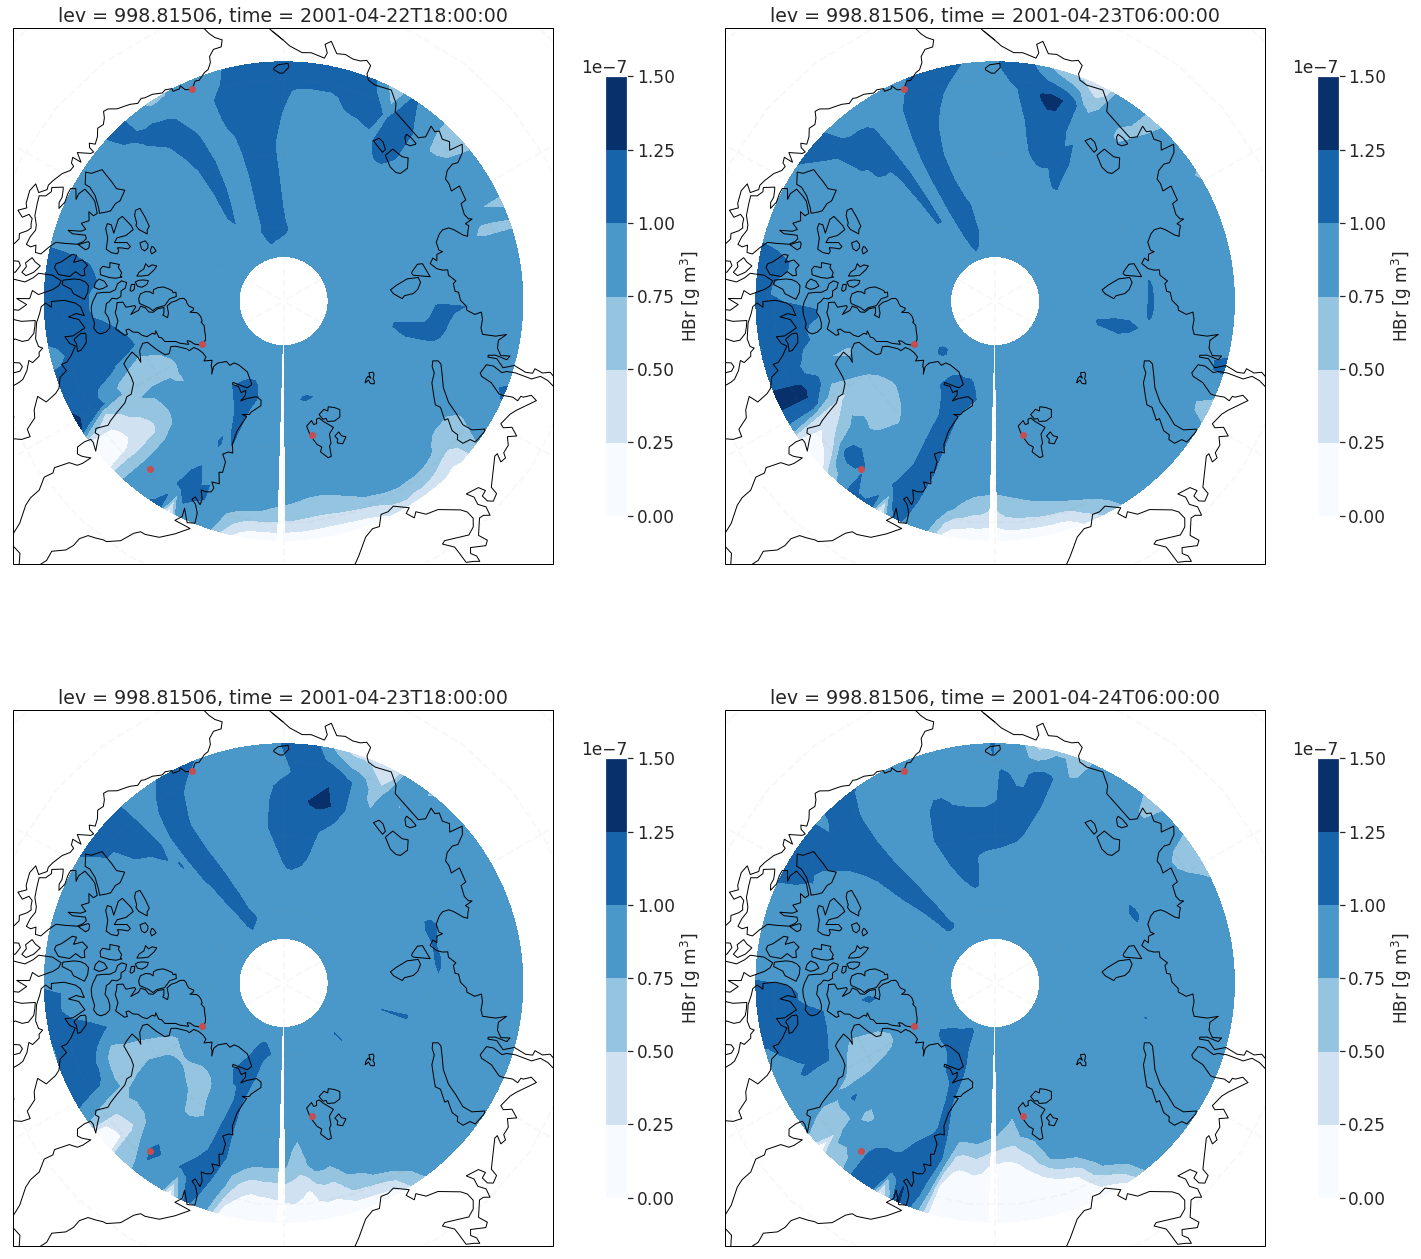
\includegraphics[width=\linewidth]{Chapter6_Results/images/polarHBr_step4.png}
    \caption{Concentration ($g m^{-3}$) of \chem{HBr} in the first model layer the Arctic at 18:00 and 06:00 (UTC) of the 22nd, 23rd and 24th of April, 2001. The result is from the test including hard-coded photodissociation rates as well as a new (high) Henry-coefficient at HFOUR resolution. The red dots are the positions of the stations with observations in 2001 (see the map in Figure \ref{fig:stns} for reference)}
    \label{fig:polarHBr_step4}
\end{figure}
\begin{figure}[h]
    \centering
    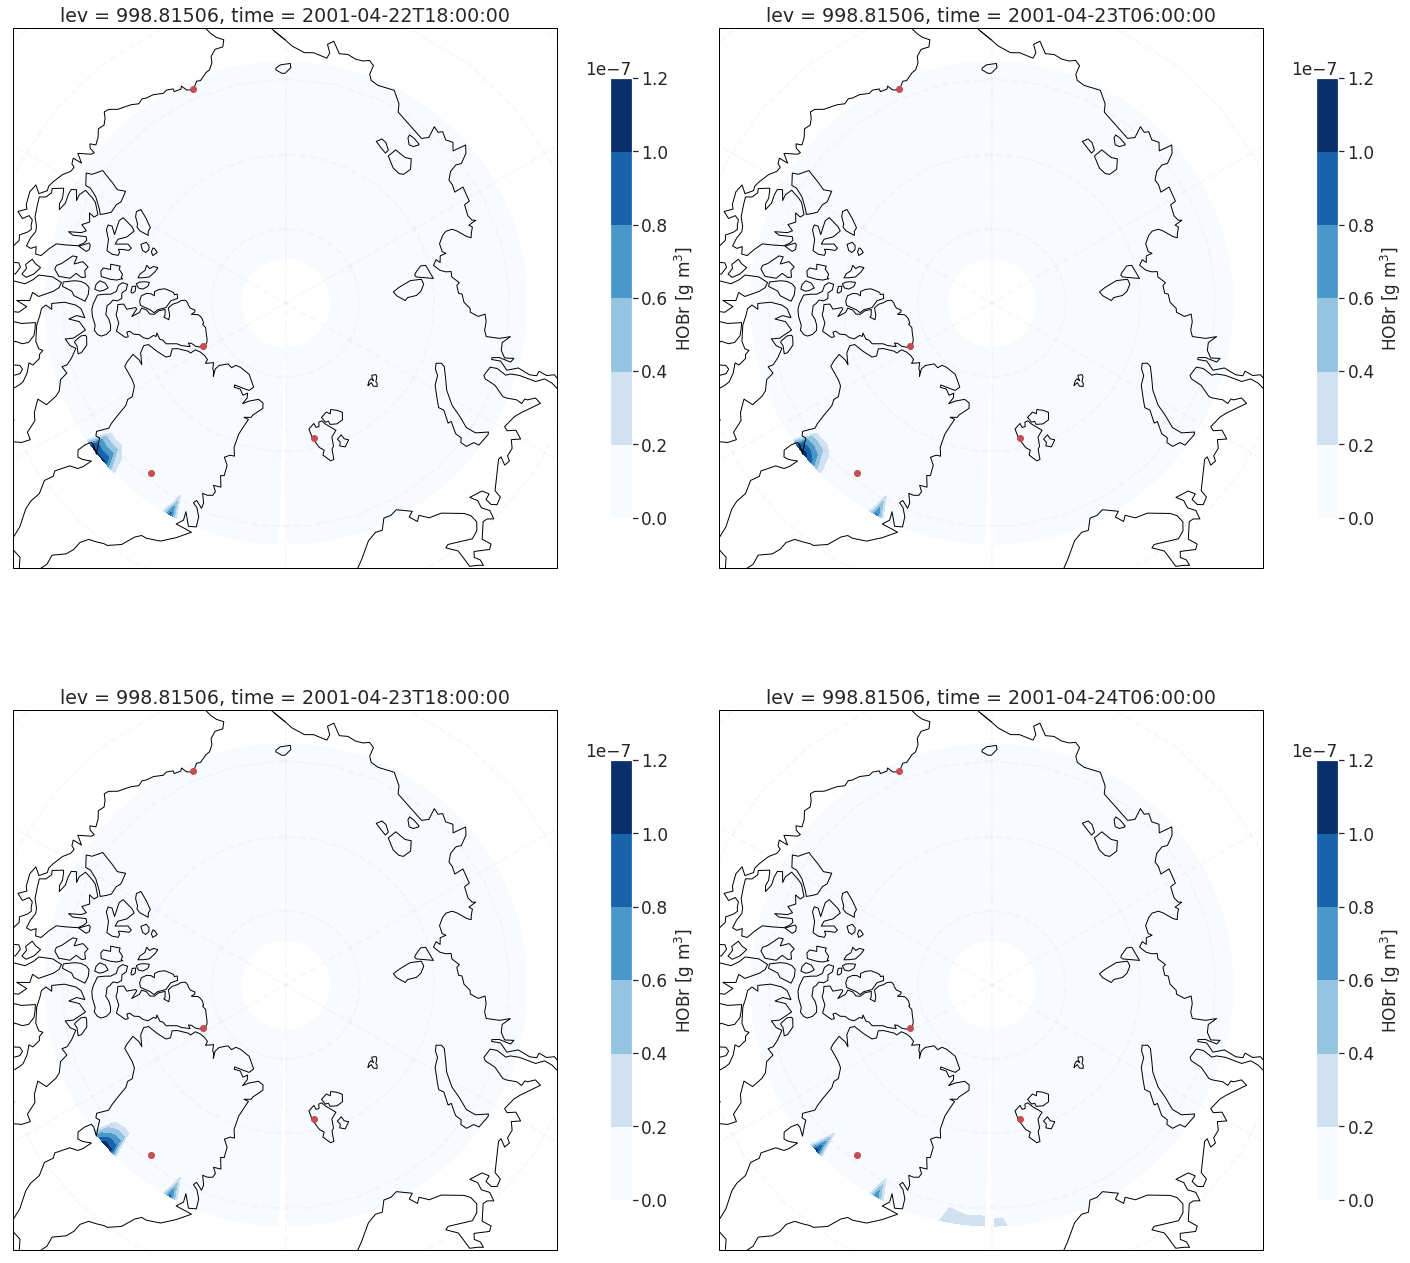
\includegraphics[width=\linewidth]{Chapter6_Results/images/polarHOBr_step4.png}
    \caption{Concentration ($g m^{-3}$) of \chem{HOBr} in the first model layer the Arctic at 18:00 and 06:00 (UTC) of the  22nd, 23rd and 24th of April, 2001. The result is from Branch \ref{def:BE_PD_noCl} initialized with a new restart file with a \chem{HBr} concentration of 10 ppt. The red dots are the positions of the stations with observations in 2001 (see the map in Figure \ref{fig:stns} for reference)}
    \label{fig:polarHOBr_step4}
\end{figure}

\medskip

The corresponding \chem{HOBr}-concentration can be seen in Figure \ref{fig:polarHOBr_step4}. Seen in relation with Figure \ref{fig:polarHBr_step4}, the anti-correlation between the \chem{HBr} and \chem{HOBr} seems to be gone, and there is practically no \chem{HOBr} in this layer. The corresponding $\chem{O_3}$-concentration can be seen in Figure \ref{fig:polarO3_step4}.

\begin{figure}[h]
    \centering
    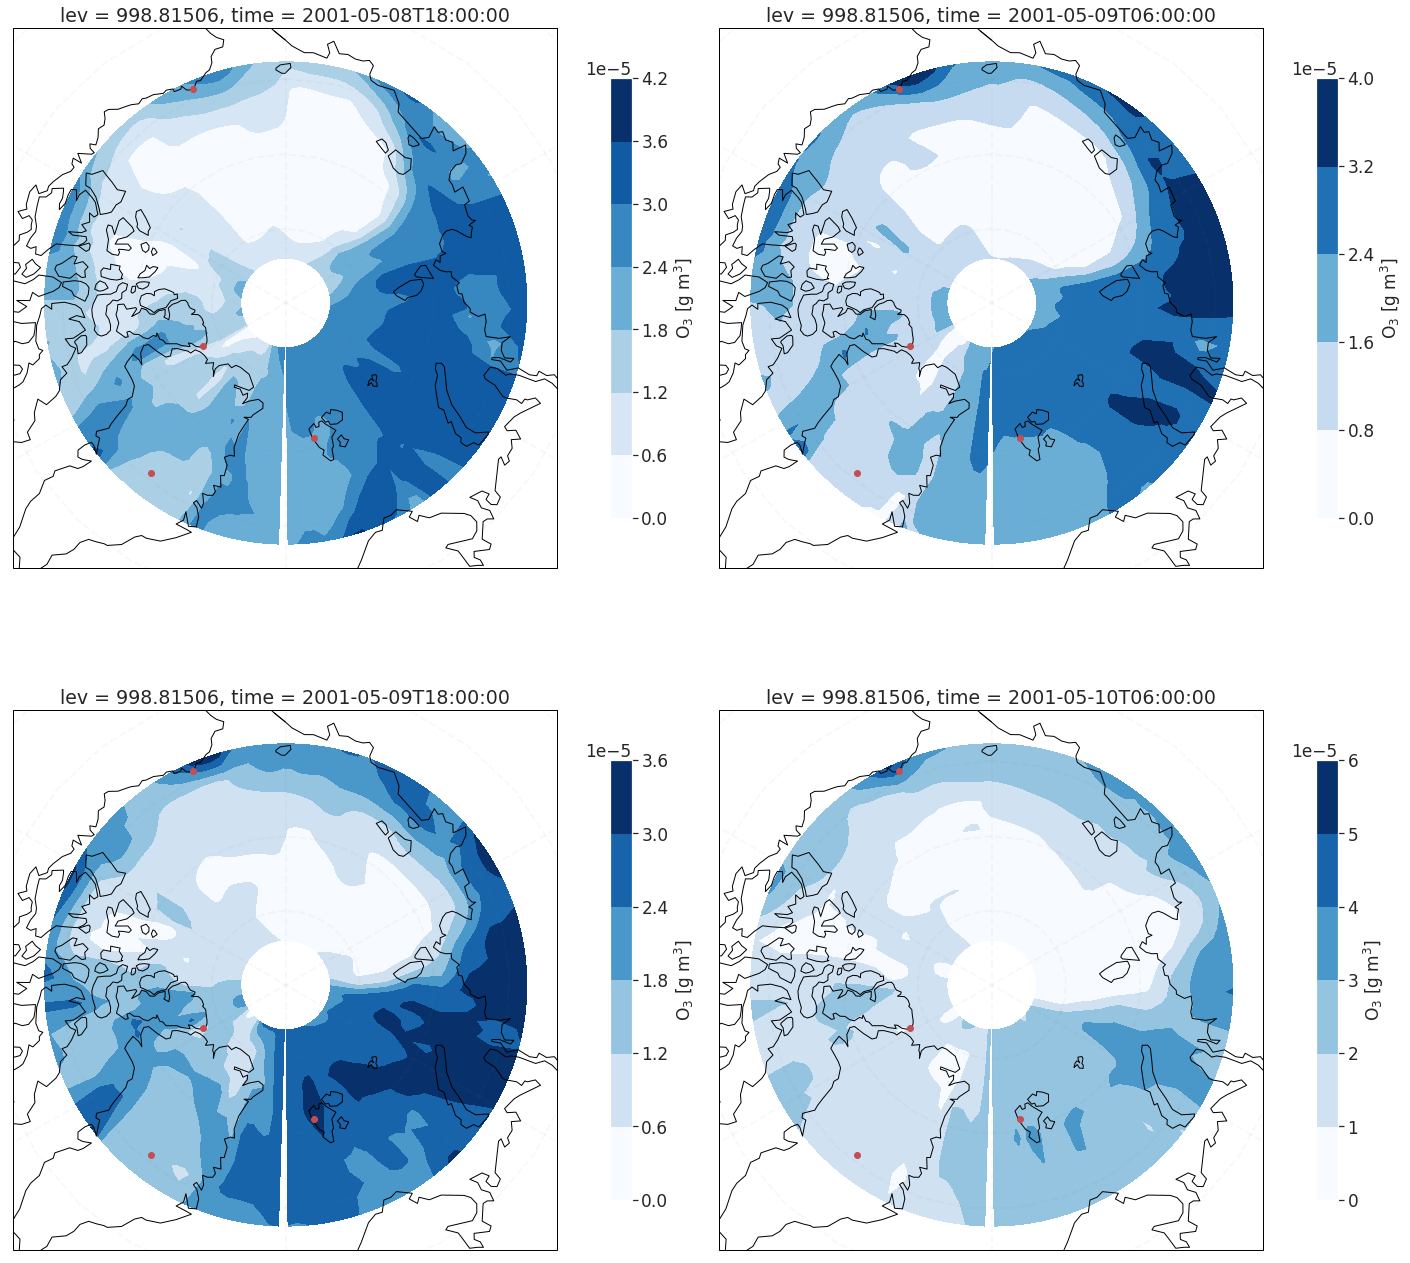
\includegraphics[width=\linewidth]{Chapter6_Results/images/polarO3_step4.png}
    \caption{Concentration ($g m^{-3}$) of $\chem{O_3}$ in the first model layer the Arctic at 18:00 and 06:00 (UTC) of the  22nd, 23rd and 24th of April, 2001. The result is from Branch \ref{def:BE_PD_noCl} initialized with a new restart file with a \chem{HBr} concentration of 10 ppt. The red dots are the positions of the stations with observations in 2001 (see the map in Figure \ref{fig:stns} for reference)}
    \label{fig:polarO3_step4}
\end{figure}

\medskip

In Figure \ref{fig:polarBrO_step4}, the resulting  \chem{BrO}-\acrshort{vcd} is on the order of $10^{8}$ molecules cm$^{-2}$. 

\begin{figure}[h]
    \centering
    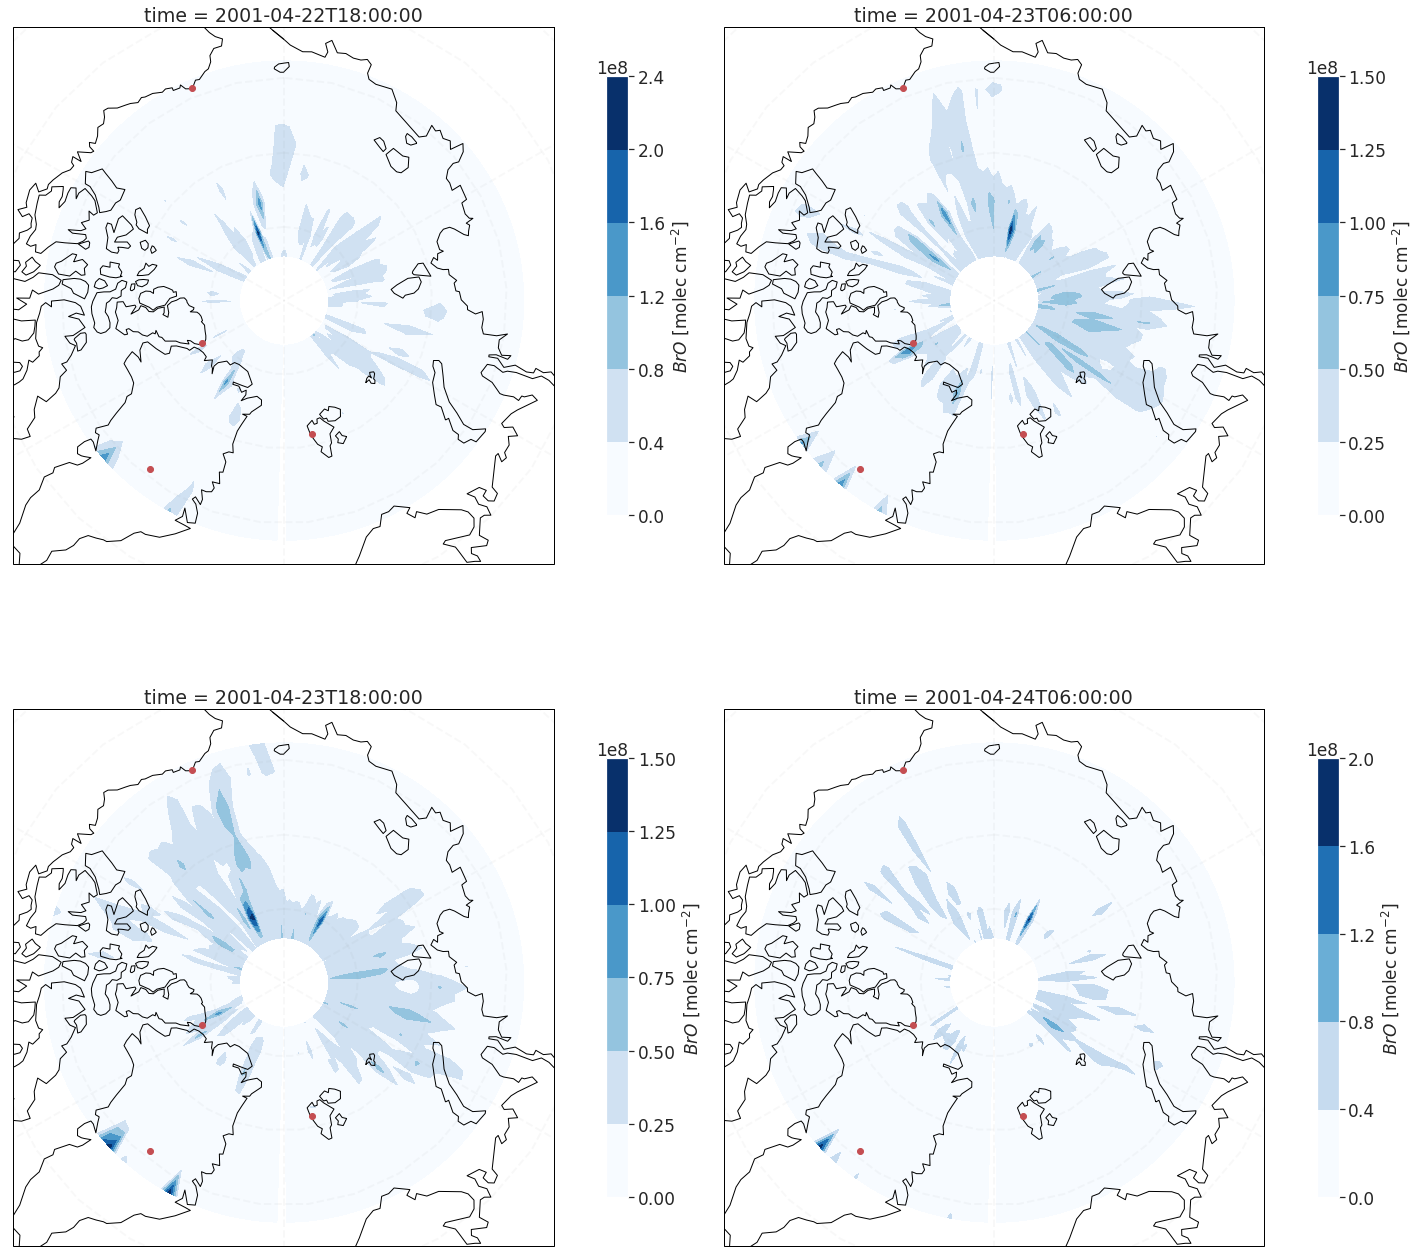
\includegraphics[width = \linewidth]{Chapter6_Results/images/polarBrO_step4.png}
    \caption{Vertical column density ($molecules cm^{-2}$) of \chem{BrO} in the lowermost $\sim 250 m$ at 18:00 and 06:00 (UTC) on the 22nd, 23rd and 24th of April, 2001. The result is from the final version of the CTM3. The red dots are the positions of the stations with observations in 2001 (see the map in Figure \ref{fig:stns} for reference)}
    \label{fig:polarBrO_step4}
\end{figure}




%\subsubsection{Changing $L_{mix}$ in Reaction \ref{R:7}}

%The boundary layer height, $L_{mix}$ and deposition velocity, $v_d$ in the preliminary runs had values listed in Section \ref{sec:impl_multiphase_react}. In an attempt to "kick-start" the bromine explosions $L_{mix}$ was lowered (And corresponding $v_d$ increased) in the \texttt{marikoll\_bromine\_explosion\_noHetChlorine}- branch. 

%\medskip

%The first test was executed with $L_{mix} = 25 m$ and $v_d = 0.00824 m/s$. This boundary layer height was chosen due to the height of the second model layer height $995.86 hPa$, with is about $23 m$ higher than the first model layer height at $998.82 hPa$. The low level was chosen to make sure the bromine explosion would indeed occur. This test caused too much bromine explosion for the model to complete the run. $L_{mix}$ was then lowered to $L_{mix} = 100 m$ with $v_d = 0.00667 m/s$. 

%\subsubsection{Lmix = 200}

%\subsubsection{Lmix = 100}

%\subsubsection{Lmix = 100 After Fix}

%The weighing of Reaction \ref{R:7} was removed (in \texttt{pchemc\_ij.f90}). It was initially weighted with $0.5$ assuming half of the \chem{HOBr} was reacting with \chem{Br} and half with \chem{Cl}, but was removed as the heterogeneous reactions involving \chem{Cl} were removed. Also, $\chem{Br_2}$ was added to the debugging-scaling in \texttt{pchemc\_ij.f90}

%\subsubsection{Lmix = 100, \chem{HBr} Adjusted to 30 ppt}

%In order to boost the concentration of \chem{HBr}, the concentration was hard-coded to 30 ppt ($= 8.059 \text{molecules}cm^{-3}$ at $273.15 K$) in the first sub-timestep of \texttt{pchemc\_ij.f90}. This worked in the test-run


%\subsubsection{Lmix = 200, \chem{HBr} Adjusted to 10 ppt}



%\subsubsection{Lmix = 100, with new restart file}

%C3RUN\_BE\_HFOUR\_HBr10ppt\_May

%Figur med HOBr og HBr - antikorrelert. Null effekt på ozon, hot spots med Br, BrO og Br2. 

%The anticorrelation of \chem{HOBr} and \chem{HBr} indicates that \chem{HOBr} is titrated from the system, leaving hot spots of \chem{HBr}. 

%\subsubsection{Lmix = 50, with new restart file}

%Still anti-correlation between \chem{HOBr} and \chem{HBr}. Maybe a bit less $\chem{O_3}$? 

%vd = 0.0074 

%C3RUN\_BE\_HFOUR\_HBr10ppt\_Lmix50\_May

%\subsubsection{Lmix = 25, with new restart file}

%vd = 0.00824

%C3RUN\_BE\_HFOUR\_HBr10ppt\_Lmix25\_May


%\subsubsection{Lmix = 100, cycling of \chem{HOBr} and \chem{HBr} and hard-coded photodissociation rates}

%C3RUN\_BE\_HFOUR\_HBr10ppt\_Lmix100\_ohbr2 - test run with the reaction: 

%\subsubsection{Test at HTWO}

%This was with both hard-coded photodissosiation rates and higher Henry coefficient C3RUN\_BE\_HTWO\_HX\_HDP\_MarchApril

%\section{Comparison between the PD- and PI-branches}

%\section{Comparison with station data}

%\section{Comparison with literature}

%\cite{Zhao2016} measured BrO column at Eureka in 2011 -- SJekk ut! 


%\cite{Peterson2016} and \cite{Peterson2015} -- BrO over Barrow -- sjekk ut! 

%Measurements of $\chem{Br_2}$, \chem{BrCl} and $\chem{O_3}$ were conducted by \cite{Foster2001} at Alert research station. They found $\chem{Br_2}$ mixing ratios up to $\sim$ 25 \acrshort{ppt} and \chem{BrCl} at mixing ratios up to 35 \acrshort{ppt} between day 40 and 75 in 2001. Ozone was depleted from background values of $\sim$ 30-40 \acrshort{ppb} to below 10 ppb. 

%\medskip

%\cite{Simpson2017} investigated the \chem{BrO} column using \acrlong{maxdoas} instrumentation near Barrow in 2012.

%\medskip

%\cite{Luo2018} also investigated the \chem{BrO} column using \acrshort{maxdoas} in Ny Ålesund in 2015. 

%\medskip

%\cite{Thomas2012} and \cite{Thomas2011} about the mechanism behind ODEs at Summit, Greenland. 

%\section{Calculation of radiative forcing using PD- and PI model results}